\documentclass[../Main.tex]{subfiles}

\begin{document}
\chapter{Wahrscheinlichkeit und Statistik}

\intro{

}

\begin{figure}[H]
    \centering
    \includegraphics[width=0.75\linewidth]{Images/lösungsansatz.png}
    \caption{Lösungsansatz von typischen WahrStat Aufgaben}
\end{figure}

\section{Kombinatorik}
Die Kombinatorik ist eine Teildisziplin der Mathematik, die sich mit endlichen oder abzählbar unendlichen diskreten Strukturen beschäftigt und deshalb auch dem Oberbegriff Diskrete Mathematik zugerechnet wird.
\defn{Produktregel (Für-jede-gibt-es-Regel)}{
Wenn es für jede von \(n\)  Wahlmöglichkeiten m mögliche weitere Wahlmöglichkeiten gibt, dann gibt es insgemsamt \(n \cdot m\)  Möglichkeiten. 
\begin{equation}
    n_1 \cdot n_2 \dots n_k = \prod_{i=1}^k n_i
\end{equation}
}

\defn{Permutation (Anordnung)}{
Gegeben sind \(n\)  anzuordnende Objekte. Die Fakultät ! beschreibt dabei die Anzahl Arten wie dies geschehen kann.
\begin{equation}
    \begin{split}
        P_n &= \#\{\text{Plätze für 1. Objekt (n)}\} \cdot \#\{\text{Plätze für 2. Objekt (n-1)}\} \cdot \\ &\dots \#\{\text{Plätze für n. Objekt (1)}\} \\
      &=  n \cdot (n-1) \dots 1 \\
      &= n!
    \end{split}
\end{equation}
}

\defn{Kombination (Auswahl Problem)}{
    Die Anzahl Objekte welche aus \(n\) von \(k\) möglichen ausgewählt werden (ohne zurücklegen) wird beschrieben durch:. 
    \begin{equation}
        \begin{split}
             \frac{n!}{k!(n-k)!} &= \binom{n}{k} \\
            \text{Binomialkoeffizient }(a+b)^n &= \sum^n \binom{n}{k}a^{n-k}b^k \\
            \text{oder auch } (1+z)^n &= \sum^n \binom{n}{k}z^k
        \end{split}
    \end{equation}
}

\defn{Variation (Perlenketten Problem)}{
   Die Arten auf welche man \(k\) mal unter \(n\) verschiedenen Objekten auswählen kann wird beschrieben durch:
   \begin{equation}
       = n \cdot n^{k-1} = n^k
   \end{equation}
}
\subsection{Erzeugende Funktion}
Ist die formale Potenzreihe einer Folge \(a_n\). Diese kann verwendet werden um Zahlen \(a_n\) in Funktionen zu codieren. Damit lassen sich kombinatorische Probleme mit algebraischer Manipulation von erzeugenden Funktionen lösen. Z.B. Gegeben 3 Einfränkler, 4 Zweifränkler und 7 Fünfliber, auf wieviele Arten kann man 39 Franken bezahlen?
\begin{equation}
    \begin{split}
        \text{1Fr } &= z \\
        \text{0-3 Einfränkler } &= f_1(z) = 1+z+z^2+z^3\\
        \text{0-4 Zweifränkler } &= f_2(z)=1+z^2+z^4+z^6+z^8\\
        \text{0-7 Fünfliber } &= f_3(z)=1+z^5+\dots +z^{35} \\
        \text{Alle } &f_1(z)\cdot f_2(z) \cdot f_5(z) = \\
        &= 1+z+2z^2+2z^3+\dots+\color{red} 4z^{23} \color{black} +  \cdots
    \end{split}
\end{equation}

\section{Ereignisse}
\defn{Elementarergeignis}{
Der Ausgang eines Experimentes heisst Elementarereignis, die Menge aller Elementarereignisse wird mit \(\Omega \) bezeichnet. Ein Elementarereignis \(\omega \) ist also ein Element von \(\Omega\), \(\omega \in \Omega \). 
}

\defn{Ereignis}{
    Ist \(\Omega \) eine Menge von Versuchsausgängen, dann heisst eine Teilmenge \( A \subset \Omega \) ein Ereignis. Man sagt, das Ereignis \(A\) ist eingetreten, wenn bei einer Durchführung des Experimentes ein Versuchsausgang \(\omega \in  A\) aufgetreten ist. 
}

\defn{Ereignisalgebra}{
    Eine Ereignisalgebra \( (\Omega , A) \) ist eine Menge \(\Omega\) mit einer Menge \(A \subset Potenzmenge(\Omega)\) von Teilmengen von \(\Omega\) , die folgende Bedingungen erfüllen: 
    \begin{enumerate}
        \item Vereinigungen von Elementen von \(A\) sind ebenfalls in \(A\), also \\
    \[B,C \in A \Rightarrow B \cup C \in A\]
        \item  Differenzen von Elementen von A sind in A, also \\
    \[ B,C \in A \Rightarrow B \setminus C \in A \]
        \item        \(\Omega \in A\) d.h. es gibt das sichere Ereignis.
    \end{enumerate}
    Sind nur die Bedingungen 1 und 2 erfüllt, spricht man auch von einem Mengen-Ring. Eine Ereignisalgebra heisst manchmal auch ein Mengenkörper. Aus den Axiomen folgt direkt:
    \begin{enumerate}
        \item Es gibt das unmögliche Ereignis: \(\emptyset\)
        \item Das Komplement eines Ereignisses ist ebenfalls ein Ereignis
        \item Der Durchschnitt zweier Ereignisse ist ebenfalls ein Ereignis.
    \end{enumerate}

    \begin{equation}
        \begin{split}
            A \cap (B \cup C) &= (A \cap B) \cup(A \cap C) \\
            A \cup (B  \cap C) &= (A \cup B) \cap (A \cup C) \\
            \overline{A \cap B} &= \bar{A}\cup\bar{B} \text{ and vice versa}
        \end{split}
    \end{equation}
}

\newpage
\section{Wahrscheinlichkeit}
Die Wahrscheinlichkeit soll ein Mass dafür sein, dass ein Ereignis eintritt. Es gibt verschiedene Ansätze, wie wir zu einem solchen Mass kommen könnten: 
\begin{enumerate}
    \item Je häufiger ein Ereignis eintritt, desto grösser sollte die Wahrscheinlichkeit sein. Dies setzt voraus, dass das Experiment im Prinzip beliebig oft wiederholbar ist. Man nennt dies den frequentistischen Ansatz. 
    \item Die Wahrscheinlichkeit ist ein Mass für die persönliche Überzeugung, dass ein Ereignis eintreten wird. Im Unterschied zum frequentistischen Ansatz sollte man bei diesem Ansatz einem Ereignis auch dann eine Wahrscheinlichkeit geben können, wenn sich ein Experiment nicht wirklich wiederholen lässt. Dies ist der Bayessche Ansatz. 
    \item Wir könnten eine Reihe von plausiblen Axiomen postulieren, nach denen sich die Wahr scheinlichkeit zu verhalten hat, und dann zu untersuchen, ob ein solches Objekt tatsäch lich existiert. Dabei ist uns egal, was der Wahrscheinlichkeitswert genau bedeutet. Dieser axiomatische Ansatz hat den Vorteil, logisch konsistent zu sein, was bei den anderen An sätzen nicht von vornherein garantiert ist. 
\end{enumerate}

In allen Fällen ergibt sich eine Reihe von Gesetzmässigkeiten oder Formeln, welche die jeweiligen Wahrscheinlichkeitsbegriffe erfüllen müssen. Soll die Wahrscheinlichkeit eine objektive Grösse sein, dann muss für wiederholbare Experimente die für den Bayesschen Ansatz nötige persönliche Überzeugung direkt mit der Häufigkeit des Eintretens zusammenhängen. Der frequentistische und der Bayessche Ansatz werden also in diesem Fall übereinstimmen. Die Axiome im axiomatischen Ansatz sind natürlich genau die Rechenregeln, die man sowohl im frequentistischen Ansatz wie auch im Bayesschen Ansatz von der Wahrscheinlichkeit erwartet. Man darf daher davon ausgehen, dass die drei Ansätze die gleichen numerischen Resultate lie fern, sie unterscheiden sich höchstens in der Interpretation der Resultate.

\defn{Wahrscheinlichkeit als relative Häufigkeit}{
\begin{equation}
    P(A)= \lim_{N \rightarrow \infty} \frac{n}{N}
\end{equation}
}

\defn{Axiome eines Wahrscheinlichkeitsraumes}{
\textbf{Wertebereich}
\begin{equation}
    0 \leq P(A) \leq 1
\end{equation}
\textbf{Sicheres Ereignis}
\begin{equation}
    P(\Omega)=1
\end{equation}
\textbf{Vereinigung}. Sind die Ereignisse \(A_1,A_2,\dots\) paarweise disjunkt. also \(A_i \cap A_j = \emptyset\) für \(i \neq j\), dann gilt
\begin{equation}
    P(A_1 \cup A2 \cup \dots)= P(A_1)+P(A_2)+\dots
\end{equation}
Aus den Axiomen folgt:
\begin{enumerate}
    \item Die Wahrscheinlichkeit des unmöglichen Ereignisses ist \\
\[P(\emptyset)=0\]
    \item Die Wahrscheinlichkeit des komplementären Ereignisses ist \\
\[ P(\bar{A}=P(\Omega \setminus A) = 1-P(A) \]
    \item Die Wahrscheinlichkeit der Differenz der Ereignisse A und B ist \\
\[ P(A \setminus B) = P(A) - P(A \cap B) \]
    \item Die Wahrscheinlichkeit der Vereinigung zweier beliebiger Ereignisse ist (Ein-/Ausschaltformel)\\
\[ P(A \cup B ) = P(A) + P(B) - P(A \cap B) \]
\end{enumerate}

}

\defn{Laplace Experiment}{
Ein Experiment mit \(n = |\Omega|\) Ausgängen heisst ein Laplace-Experiment, wenn jeder Versuchsausgang gleich wahrscheinlich mit Wahrscheinlichkeit 
\begin{equation}
    P(\omega) = \frac{1}{n}, w\in \Omega
\end{equation}
\begin{equation}
    P(A)=\frac{|A|}{|\Omega|}
\end{equation}
Nur das unmögliche Ereignis hat Wahrscheinlichkeit 0.
}
\defn{Bernoulli Experiment}{
Genau zwei Versuchsausgänge mit Wahrscheinlichkeiten \(p\) und \(1-p\). 
}

\defn{Bedingte Wahrscheinlichkeit}{
Die bedingte Wahrscheinlichkeit eines Ereignisses A unter der Bedingung B ist 
\begin{equation}
    P(A|B)=\frac{P(A \cap B)}{P(B)}
\end{equation}
Man liest dies auch als “Wahrscheinlichkeit von A bedingt B”.
}

\defn{Unabhängigkeit}{
    Die Ereignisse A und B heissen unabhängig, wenn gilt:
    \begin{equation}
        P(A \cap B) = P(A) \cdot P(B)
    \end{equation}
}

\defn{Satz der totalen Wahrscheinlichkeit}{
    Ist \(B_i\) eine Folge paarweise disjunkter Mengen mit \( \bigcup_{i=0}^n B_i = \Omega \) , dann gilt für jedes Ereignis \(A\) 
    \begin{equation}
        P(A)= \sum_{i=0}^n P(A|B_i) \cdot P(B_i)
    \end{equation}
}

\subsection{Bayesischer Ansatz}
%tbd explain some more
\defn{Satz von Bayes}{
    Für zwei beliebige Ereignisse mit \(A\) und \(B\) mit nicht
    verschwindender Wahrscheinlichkeit \(P(B) \neq 0\) gilt 
    \begin{equation}
        \begin{split}
            P(A|B) \cdot P(B) = P(A \cap B) = P(B|A) \cdot P(A),\\
            P(A|B)= \frac{P(B|A) \cdot P(A)}{P(B)}
        \end{split}
    \end{equation}
}

\subsection{Google Matrix}

\section{Zufallsvariable}
In der Stochastik ist eine \textbf{Zufallsvariable} (auch \textbf{zufällige Variable}, \textbf{zufällige Größe}, \textbf{zufällige Veränderliche}, \textbf{zufälliges Element}, \textbf{Zufallselement}, \textbf{Zufallsveränderliche}) eine Größe, deren Wert vom Zufall abhängig ist. Formal ist eine Zufallsvariable eine Funktion, die jedem möglichen Ergebnis eines Zufallsexperiments eine Größe zuordnet. Ist diese Größe eine reelle Zahl, so spricht man von einer \textbf{reellen Zufallsvariablen} oder \textbf{Zufallsgröße}. Beispiele für reelle Zufallsvariablen sind die Augensumme von zwei geworfenen Würfeln und die Gewinnhöhe in einem Glücksspiel. Zufallsvariablen können aber auch komplexere mathematische Objekte sein, wie Zufallsfelder, Zufallsbewegungen, Zufallspermutationen oder Zufallsgraphen. Über verschiedene Zuordnungsvorschriften können einem Zufallsexperiment auch verschiedene Zufallsvariablen zugeordnet werden.
\defn{Zufallsvariable}{
    Eine Zufallsvariable ist eine Funktion \(Q \rightarrow \mathbb{R} \) .
    Eine diskrete Zufallsvariable nimmt nurdiskrete Werte in \( \mathbb{R}\) an.
    Bei einer stetigen Zufallsvariable sind beliebige Werte \(X(\omega) \in \mathbb(R)\)
    möglich. Mit der zusätzlichen Eigenschaft , dass die Mengen
    \(\{\omega|X(\omega) < x\}\) Ereignisse sind. 
    \\\\
    Mit einer Zufallsvariablen \(X\) kann man wieder neue Ereignisse definieren.
    \begin{equation}
        \begin{split}
            \{X=a\} = \{ \omega \in \Omega | X(\omega) = a \} \\
            \{a < X\leq b \} = \{ \omega \in \Omega | a < X(\omega) \leq b \}
        \end{split}
    \end{equation}
    Bei einer stetigen Zufallsvariable sind die Ereignisse der Form \(\{X = a\}\) 
    nur von beschränktem Nutzen, da nur ganz wenige Versuche dazu führen werden, 
    dass das Ereignis eintritt. 
}

Die Zufälligkeit liegt in dem Versuch, der das \(\omega\) ermittelt.
Die Zuweisung des Wertes \(X(\omega)\) ist deterministisch.

\begin{figure}[H]
    \centering
    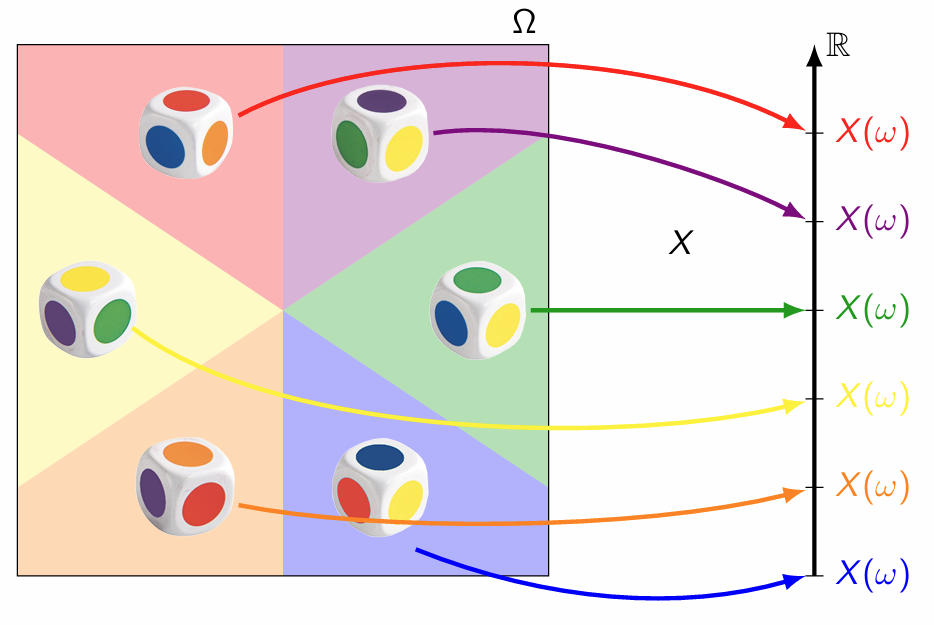
\includegraphics[width=0.75\linewidth]{Images/zufallsvariable.png}
    \caption{Die Zufallsvariable}
\end{figure}

\defn{Zufallsvariable und Wahrscheinlichkeiten}{
    Die Zufallsvariable \(X\) definiert neue Ereignisse:
    \begin{equation}
        \begin{split}
                P(X=a) &= P(\{ \omega \in \Omega | X(\omega)=a\}) \\
                &=P(\{X=a\}) \\
                P(X \leq a) &= P(\{\omega \in \Omega | X(\omega) \leq a\}) \\
                &= P(\{X \leq a\}) \\
                P(a < X \leq b) &= P(\{a < X \leq b\})
        \end{split}
    \end{equation}
}

\subsection{Diskret oder Stetig}
Eine Zufallsvariable heisst \textbf{diskret}, wenn sie
nur einzelne genau bestimmte Zahlenwerte
\(x_1, x_2,x_3,\dots\) annehmen kann.

Eine Zufallsvariable heisst \textbf{stetig}, wenn sie
beliebige Werte in einem Intervall
annehmen kann (Wertemenge ist nicht
diskret)

\defn{Einzelwahrscheinlichkeit von stetigen Zufallsvariabeln}{
    Spezifische Einzelwerte haben in einer diskreten Zufallsvariabel
    die Wahrscheinlichkeit 0.
    \begin{equation}
        P(X = x) = 0
    \end{equation}
}

\subsection{Abhängigkeit}
\defn{Unabhängigkeit}{
    Zwei Zufallsvariable \(X\) und \(Y\) heissen unabhängig,
    wenn die Ereignisse \(\{\omega|X(\omega) \leq x\}\) und
    \(\{\omega|Y(\omega) \leq y\}\) für alle \(x,y \in \mathbb{R}\)
    unabhängig sind, also
    \begin{equation}
        P((X \leq x)  \land (Y \leq y)) = P(X \leq x) P(Y \leq y) \quad \forall x, y \in \mathbb{R}
    \end{equation}
}
Das bedeutet, dass zwei Ereignisse \(A_i, B_j\),
auf denen \(X\) bzw. \(Y\) konstant ist \(\Rightarrow\) unabhängig.


\begin{figure}[H]
    \centering
    \includegraphics[width=1\linewidth]{Images/unkorreliert_unabhängig.png}
    \caption{Unkorreliert - Unabhängig}
\end{figure}

\section{Erwartungswert}
\begin{figure}[H]
    \centering
    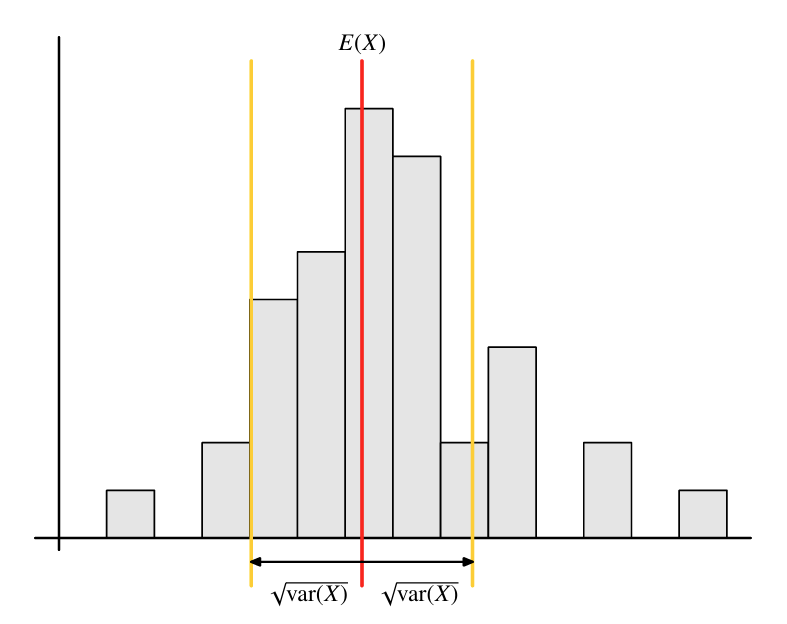
\includegraphics[width=1\linewidth]{Images/erwartungswert-varianz.png}
    \caption{Darstellung von Erwartungswert und Varianz}
\end{figure}
Der \textbf{Erwartungswert}
(selten und doppeldeutig Mittelwert)
ist ein Grundbegriff der Stochastik.
Der Erwartungswert ist eine Kennzahl einer Zufallsvariablen.
Bei einer engeren Definition ist der Erwartungswert einer Zufallsvariablen eine reelle Zahl und damit endlich;
bei einer weiteren Definition sind für den Erwartungswert einer Zufallsvariablen auch die Werte \(\pm \infty\) zugelassen.
Es gibt Zufallsvariablen, für die kein Erwartungswert definiert ist. 
\defn{Erwartungswert}{
Sei \(X\) eine Funktion auf \(\Omega\) , und lasse sich \(\Omega\) in endlich viele Ereignisse \(A_i\) zerlegen, auf denen \(X(\omega)\) konstant ist, dann ist der Erwartungswert von \(X\) 
\begin{equation}
    E(X)=\sum_{i=0}^n P(A_i) \cdot X(A_i)
\end{equation}
\textbf{Der Erwartungswert einer reelen Zufallsvariable ist diejenige Zahl, für die die Varianz minimal wird.}

Sind \(X\) und \(Y\) Zufallsvariable mit Werten in \(\mathbb{R}\) , und \(\lambda\), dann gilt
\begin{enumerate}
    \item \( E(X+Y) = E(X) + E(Y) \)
    \item \( E(\lambda X) = \lambda E(X) \)
    \item Sei \(X_A\) die charakteristische Funktion des Ereignisses \(A \in \mathbb{A}\) , welche definiert ist durch
\[ X_A: \Omega \rightarrow \mathbb{R}: \omega \mapsto	 \begin{cases}
    1 \quad \omega \in A \\
    0 \quad \omega \notin A
\end{cases}\]
dann gilt \(E(X_A)=P(A)\).
\end{enumerate}
}

\subsection{Unabhängigkeit}
\defn{Erwartungswert Produkregel (bei Unabhängigkeit)}{
Sind X und Y \textbf{unabhängige} Zufallsvariablen, dann gilt 
\[ E(XY) = E(X) \cdot E(Y) \]
}
\begin{figure}[H]
    \centering
    \includegraphics[width=0.75\linewidth]{Images/erwartung_unabhängigkeit.png}
    \caption{Unabhängigkeit}
    \label{fig:Erwartungswert-Unabhängigkeit}
\end{figure}

\subsection{Empirischer Erwartungswert}
\defn{Empirischer Erwartungswert}{
    Mit der empirischen Wahrscheinlichkeit:
    \begin{equation}
        P(X=x_i) = \frac{n_i}{n}
    \end{equation}
    Lässt sich der empirische Erwartungswert berechnen:
    \begin{equation}
        \approx \sum_{i} x_i \frac{n_i}{n}
    \end{equation}
}

\subsection{Verbindung zur Wahrscheinlichkeit}
Bei einem Ergebnis \(A \subset \Omega\), dann kann eine Funktion gebildet werden,
die \textbf{charakteristische Funktion}, welche \(A\) wie folgt abbildet:
\begin{equation}
    \chi_A : \begin{cases}
        \Omega &\to \mathbb{R} \\
        \omega &\mapsto \chi_A(\omega) \begin{cases}
            1 & \omega \in A\\
            0 & \omega \notin A
        \end{cases}
    \end{cases}
\end{equation}
Ihr Erwartungswert ist somit:
\defn{Erwartungswert der charakteristischen Funktion}{
    \begin{equation}
        E(\chi_A) = 1 \cdot P(A) + 0 \cdot (1-P(A)) = P(A)
    \end{equation}
}

\subsection{Rechenregeln}
Der Erwartungswert ist linear.
\defn{Rechenregeln}{
    Sind \(X,Y\) Zufallsvaribeln, dann gilt:
    \begin{equation}
        \begin{split}
            E(X+Y) &= E(X) + E(Y) \\
            E(\lambda X) &= \lambda E(X)
        \end{split}
    \end{equation}
}

\newpage
\section{Varianz}
Die \textbf{Varianz} (lateinisch \textit{variantia} „Verschiedenheit“ bzw.
\textit{variare} „(ver)ändern, verschieden sein“) ist ein zentrale Moment
zweiter Ordnung einer Zufallsvariablen. 

\defn{Varianz}{
Sei \(X: \Omega \rightarrow \mathbb{R}\)  eine Zufallsvariable, dann
heisst die durch \(var(X)^2 = E((X-E(X))^2) \) definierte Grösse var(X)
die Varianz von X. Oder auch die mittlere quadratische Abweichung vom
Erwartungswert. Es ist insbesondere
\begin{equation}
    var(X) = E((X-E(X))^2) = E(X^2) - E(X)^2
\end{equation}

Man beachte, dass \(var(X)\) die Masseinheit des Quadrates von \(X\) hat.
Wenn also \(X\) als Masseinheit eine Länge hat, dann hat \(var(X) \)
die Masseinheit einer Fläche. Insbesondere kann man \(var(X)\) nicht in
der gleichen Zeichnung visualisieren wie \(E(X)\). Aber die Grösse
\(\sqrt{var(X)}\) hat die gleiche Masseinheit, sie drückt die "Streubreite"
der Werte von \(X\).
}

\defn{Rechenregeln}{
Seien \(X\) und \(Y\) unabhängige Zufallsvariable, dann haben Summe und Produkt folgende Varianz
\begin{equation}
    \begin{split}
        var(\lambda X) &= \lambda^2 var(X) \\
        var(X+Y) &= var(X) + var(Y) \\
        var(XY) &= var(X) var(Y) + var(Y)E(X)^2 + var(X) E(Y)^2
    \end{split}
\end{equation}
}

\subsection{Kovarianz}
\defn{Kovarianz}{
    Die Kovarianz wird als Korrelationsmass benutzt, diese ist definiert als:
    \begin{equation}
        cov(X,Y) = E(XY) - E(X) E(Y)
    \end{equation}
}

\subsection{Empirische Varianz}{
    Für Messwerte \(x_1, \dots, x_n\) einer Zufallsvariable \(X\),
    ist die empirische Varianz definiert als:
    \begin{equation}
        var(X) \approx \frac{1}{n} \sum_{i=1}^{n} (x_i- \varphi)^2
    \end{equation}
}
Für einen noch genaueren Schätzer, benutzt man die Stichproben varianz, welche erwartungstreu ist:
\defn{Schätzer für die empirische Varianz}{
    \begin{equation}
        S^2 = \frac{1}{n-1} \sum_{i=1}^{n} (X_i - \bar{X})^2
    \end{equation}
}
\newpage

\section{Bewertung vom Mittelwert / Erwartungswert}

\subsection{Tschebyscheff}
\begin{figure}[H]
    \centering
    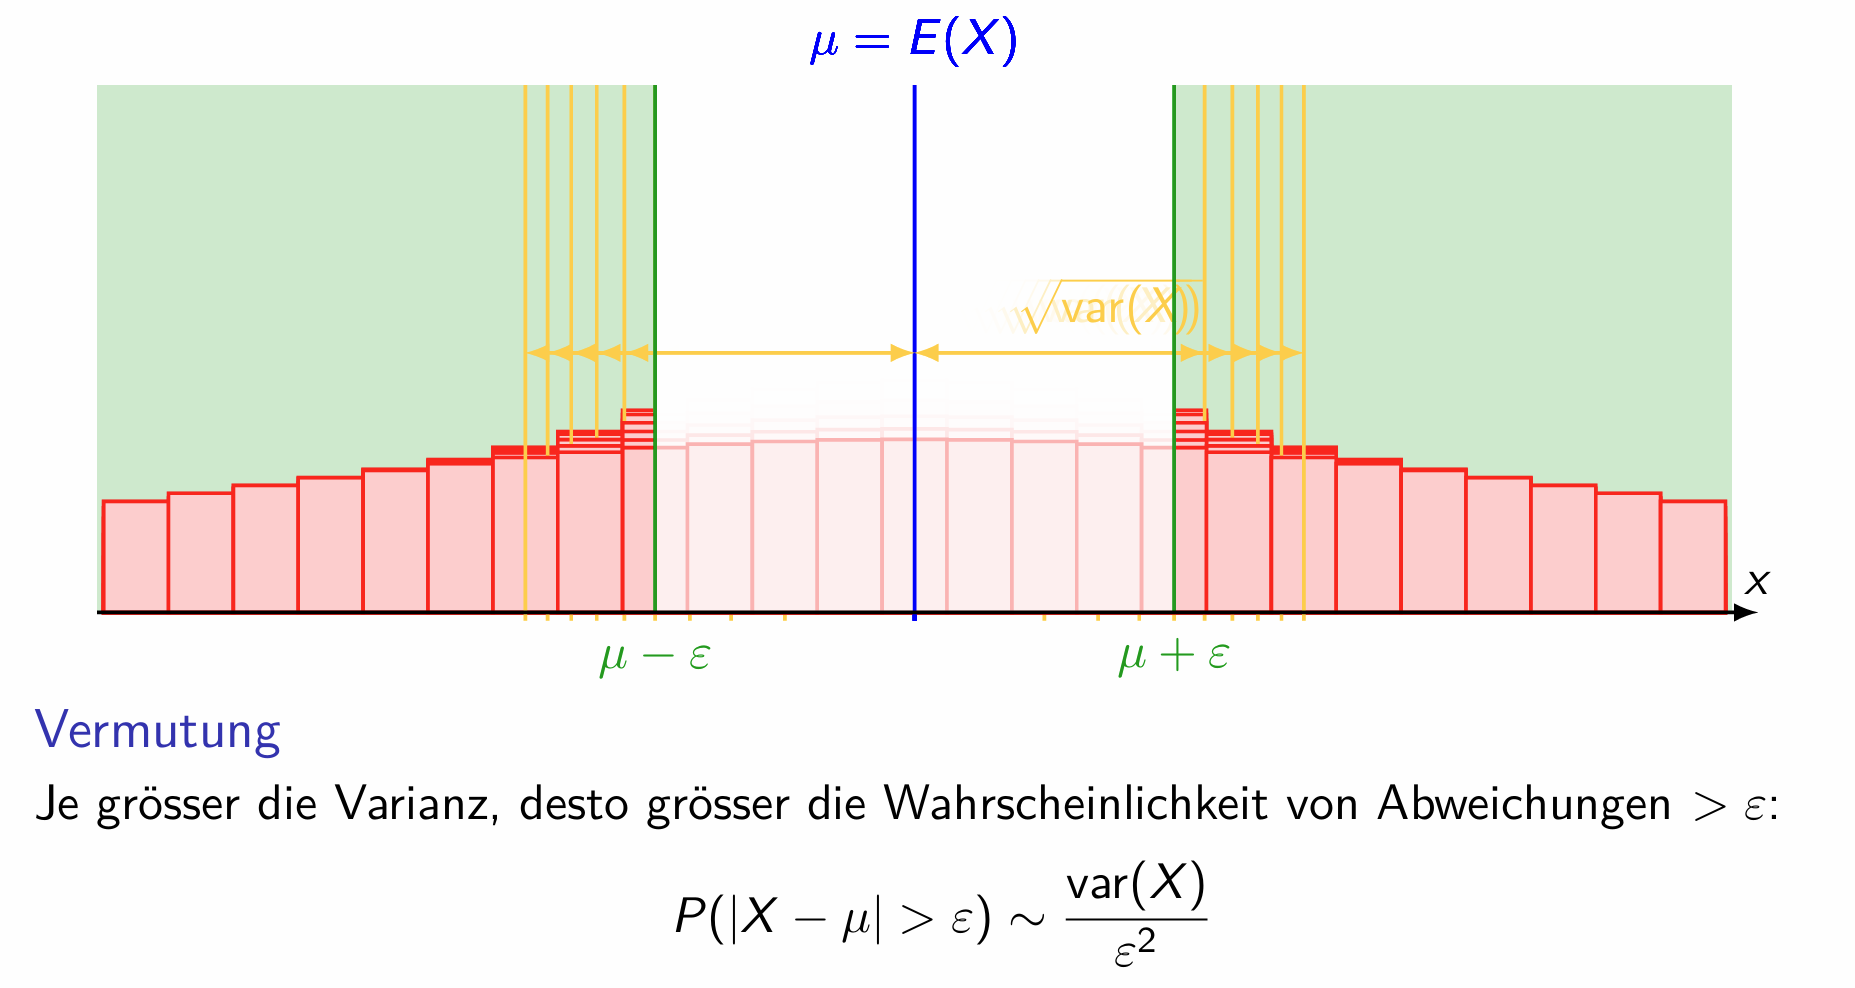
\includegraphics[width=1\linewidth]{Images/tschebyschef.png}
    \caption{Anwendung Tschebyschef}
\end{figure}

\defn{Tschebyscheff Ungleichung}{
    \(X\) eine Zufallsvariable mit Erwartungswert \(\mu = E(X)\),
    dann lässt sich die Wahrscheinlichkeit, dass \(X\) um mehr als
    \(\epsilon\) vom Erwartungswert abweicht, wie folgt abschätzen: 
    \begin{equation}
        P(|X- \mu| > \varepsilon) \leq \frac{var(x)}{\varepsilon^2}
    \end{equation}
}
Lässt man \(\varepsilon\) wachsen findet man,
dass Abweichungen deutlich grösser als \(\sqrt{var(X)}\) unwahrscheinlich sind.  
Leider sind die Vorhersagen wie auch bei der
Tschebyscheff-Ungleichung nur beschränkt nützlich.
Wenn die Wahrscheinlichkeit, dass der Mittelwert um mehr
als \(\sigma\) vom Erwartungswert abweicht, kleiner als
\textbf{1\% } sein soll, sind dafür nach dem Gesetz der grossen Zahlen
mindestens \textbf{100 Summanden nötig}. 

\begin{figure}[H]
    \centering
    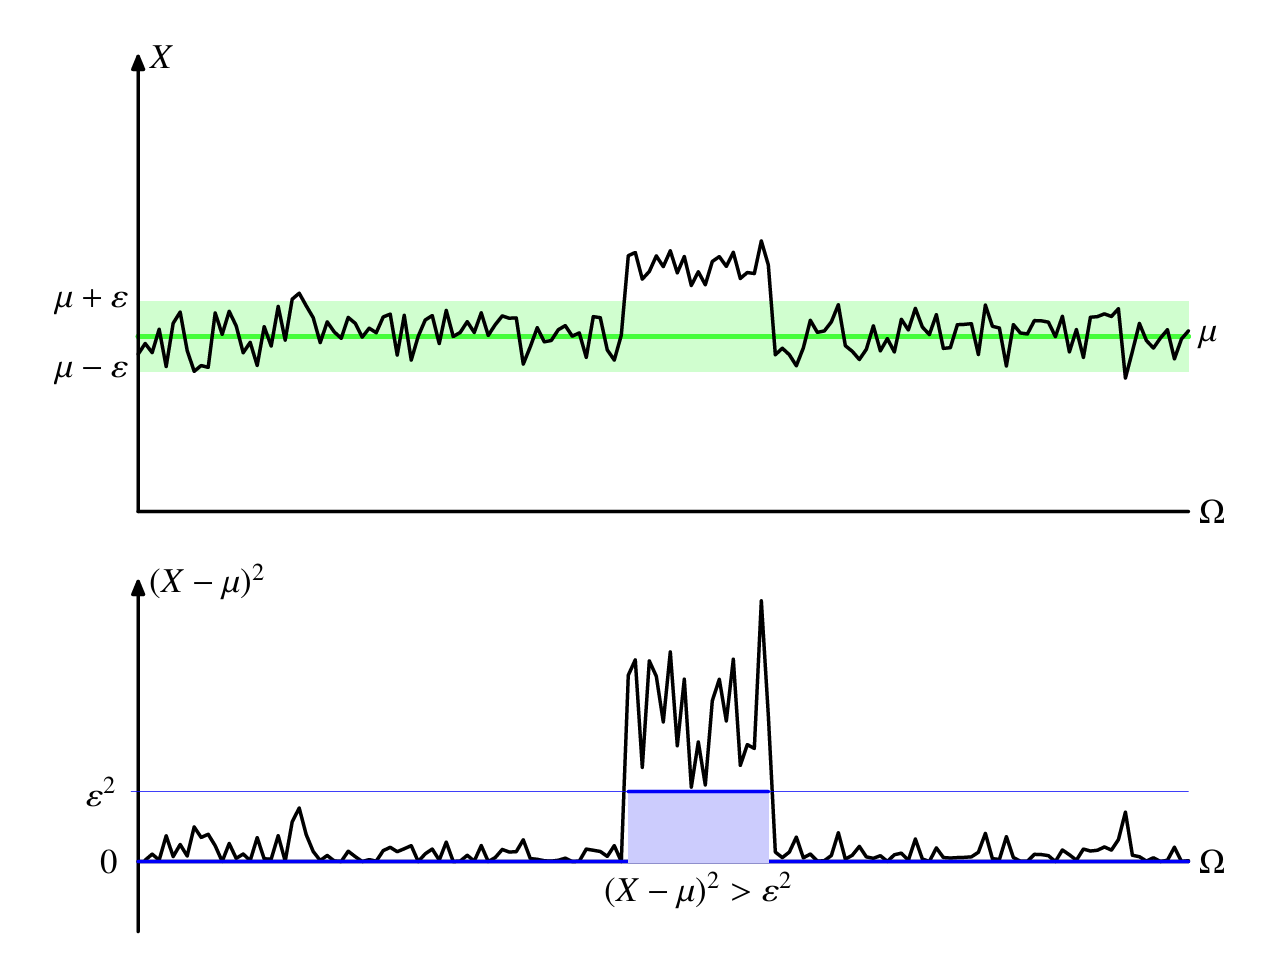
\includegraphics[width=0.75\linewidth]{Images/Tschebyscheff-Ungleichung.png}
    \caption{Herleitung der Tschebyscheff-Ungleichung, charakteristische Funktion des Er eignisses |X - µ| > \(\epsilon\) ist blau eingezeichnet. }
\end{figure}

\newpage
\subsection{Bernoulli}
\defn{Bernoulli Gesetz der grossen Zahlen}{
    Die Wahrscheinlichkeit, dass der Mittelwert von \(n\)
    unabhängigen Zufallsvariablen mit Erwartungswert \(\mu\)
    und Varianz \(\sigma^2\) mehr als \(\varepsilon\) von \(\mu\) abweicht, ist :
    \begin{equation}
        P(|M_n - \mu| > \varepsilon) \leq \frac{var(X)}{n\varepsilon^2}
    \end{equation}
    Insbesondere gilt
    \begin{equation}
        \lim_{n \rightarrow \infty} P(|M_n - \mu| > \varepsilon) = 0
    \end{equation}
}

\defn{Genauigkeit der empirischen Häufigkeit}{
    Wird ein Experiment \(n\) mal durchgeführt, und tritt dabei das
    Ereignis \(A\) mit der relativen Häufigkeit \(h\)  ein, dann ist
    die Wahrscheinlichkeit, dass \(h\) um mehr als  \( \varepsilon\)
    von \(P(A)\) abweicht
    \begin{equation}v
        P(|h-P(A)| > \varepsilon ) \leq  \frac{P(A)(1-P(A))}{n \varepsilon^2} \leq \frac{1}{4n \varepsilon^2}
    \end{equation}
}

\newpage
\section{(Einfache) Lineare Regression }
Für weitere Informationen siehe Teil "Data Science".
Die Abweichung eines Punktes beschreiben wir mit:
\begin{equation}
    \Delta = Y-(aX+b)
\end{equation}

\begin{figure}[H]
    \centering
    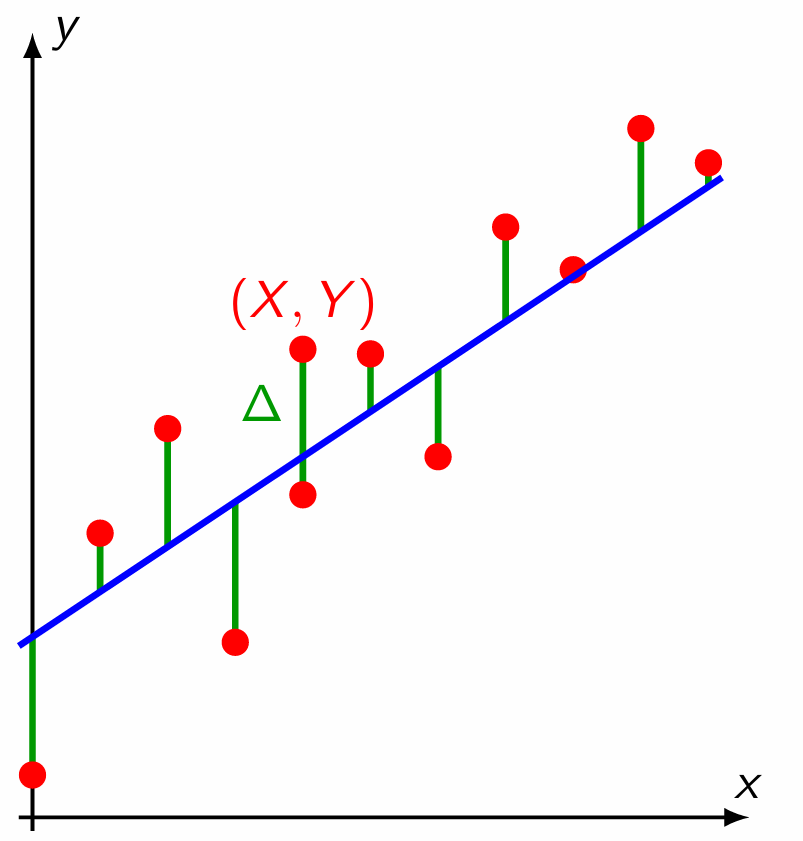
\includegraphics[width=0.5\linewidth]{Images/lineare-regression.png}
    \caption{Lineare Regression}
\end{figure}

Wir möchten nun den gemittelten Fehler minimieren. Dies lässt sich veranstalten,
wenn das \(\Delta\) quadriert wird und wir den Erwartungswert betrachten, denn:
\begin{equation}
    |\Delta| = (Y-aX-b)^2 \Rightarrow E(\Delta^2) = E((Y-aX-b)^2) = var(\Delta)
\end{equation}
Wir möchten also die Koeffizienten der linearen Funktion bestimmen, sodass
die Varianz vom mittleren Fehler resp. erwarteten Fehler minimal wird. Den 
mittleren Fehler betitelt man auch als MSE (Mean Squared Error).

Durch Lösen des Optimierungsproblems erhält man die Koeffizienten:
\defn{Lösung für Koeffizienten}{
    \begin{equation}
        \begin{split}
            a &= \frac{E(XY)-E(X)E(Y)}{E(X^2)-E(X)^2} = \frac{cov(X,Y)}{var(X)} \\
            b &= E(Y)-aE(X)
        \end{split}
    \end{equation}
}

\subsection{Fehler}
\defn{Fehlerberechnung}{
    \begin{equation}
        \begin{split}
            var(Y-aX-b) &= \dots \\
            &=\frac{var(Y-aX-B)}{var(Y)} = 1 - \frac{cov(X,Y)^2}{var(X)var(Y)} = 1 - r^2\\
            \text{Gut für } r^2 &\simeq 1 \\
            \text{Berechnung: } &= \frac{E(XY)-E(X)E(Y)}{\sqrt{var(X)var(Y)}}
        \end{split}
    \end{equation}
    \(r^2\) hängt symmetrisch von \(X\) und \(Y\) ab.
}
\subsection{Andere Basisfunktionen}
\begin{figure}[H]
    \centering  %angle=90,
    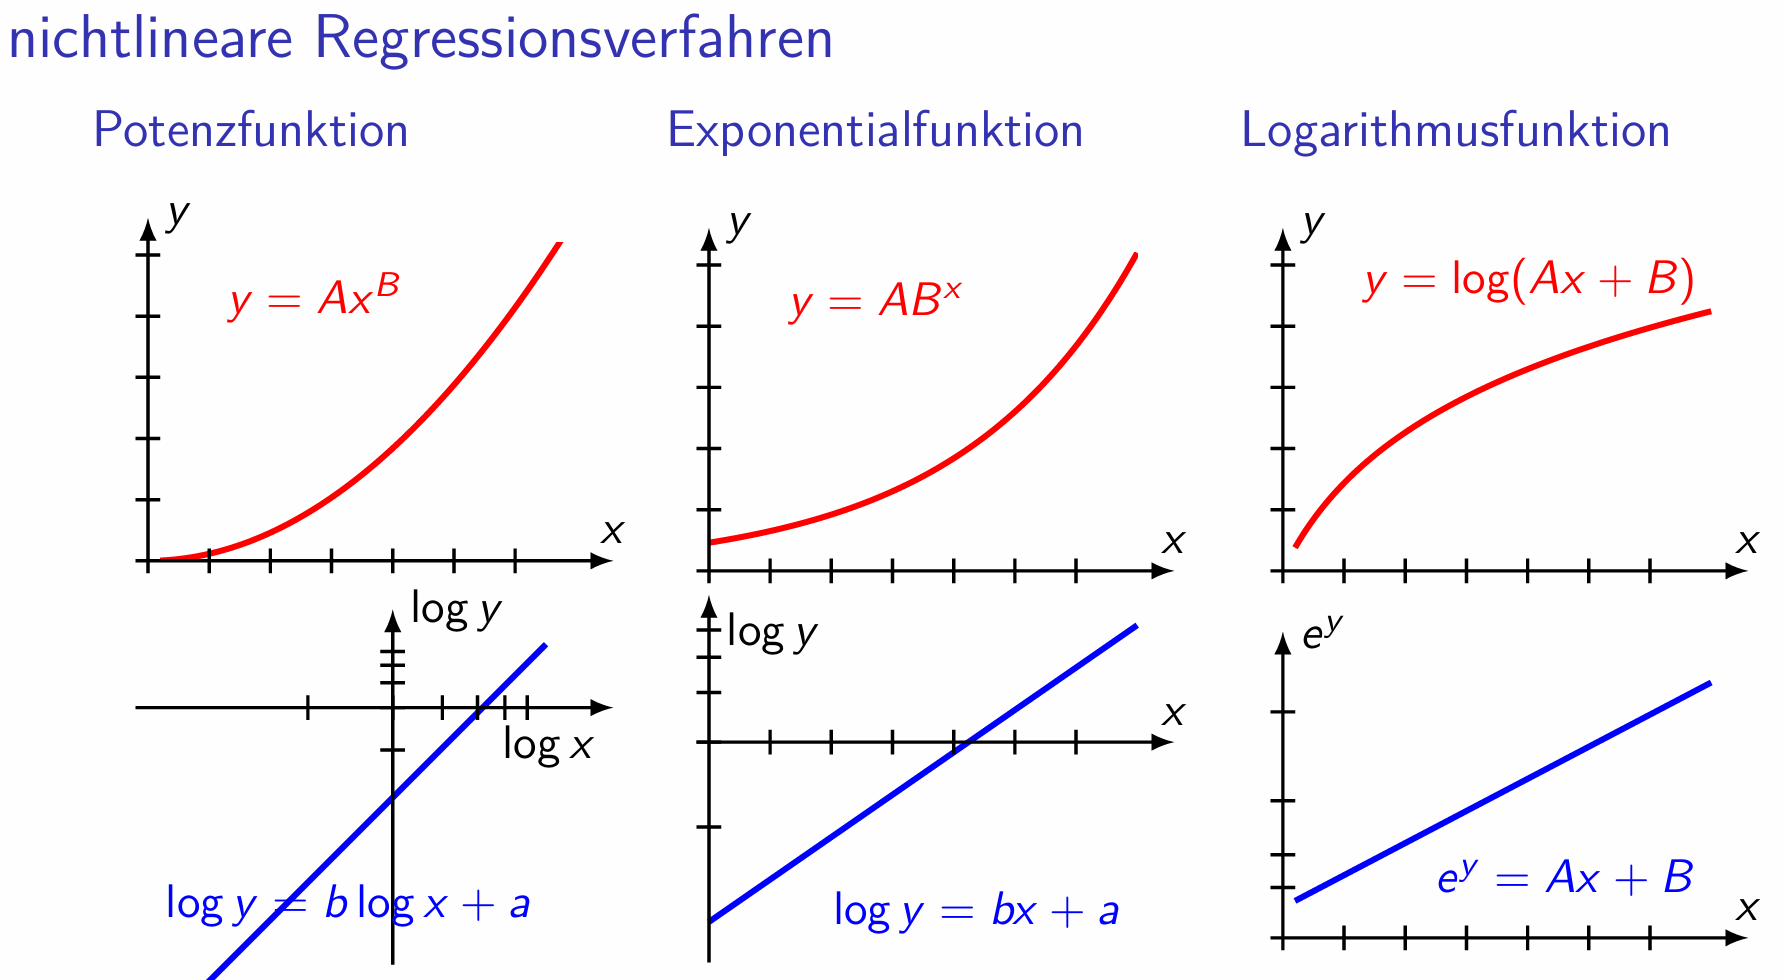
\includegraphics[height=0.5\textwidth]{Images/nichtlineare_regression.png}
    \caption{(Nicht)Lineare Regression}
\end{figure}
\newpage
\subsection{Vorlage}
\begin{figure}[H]
    \centering
    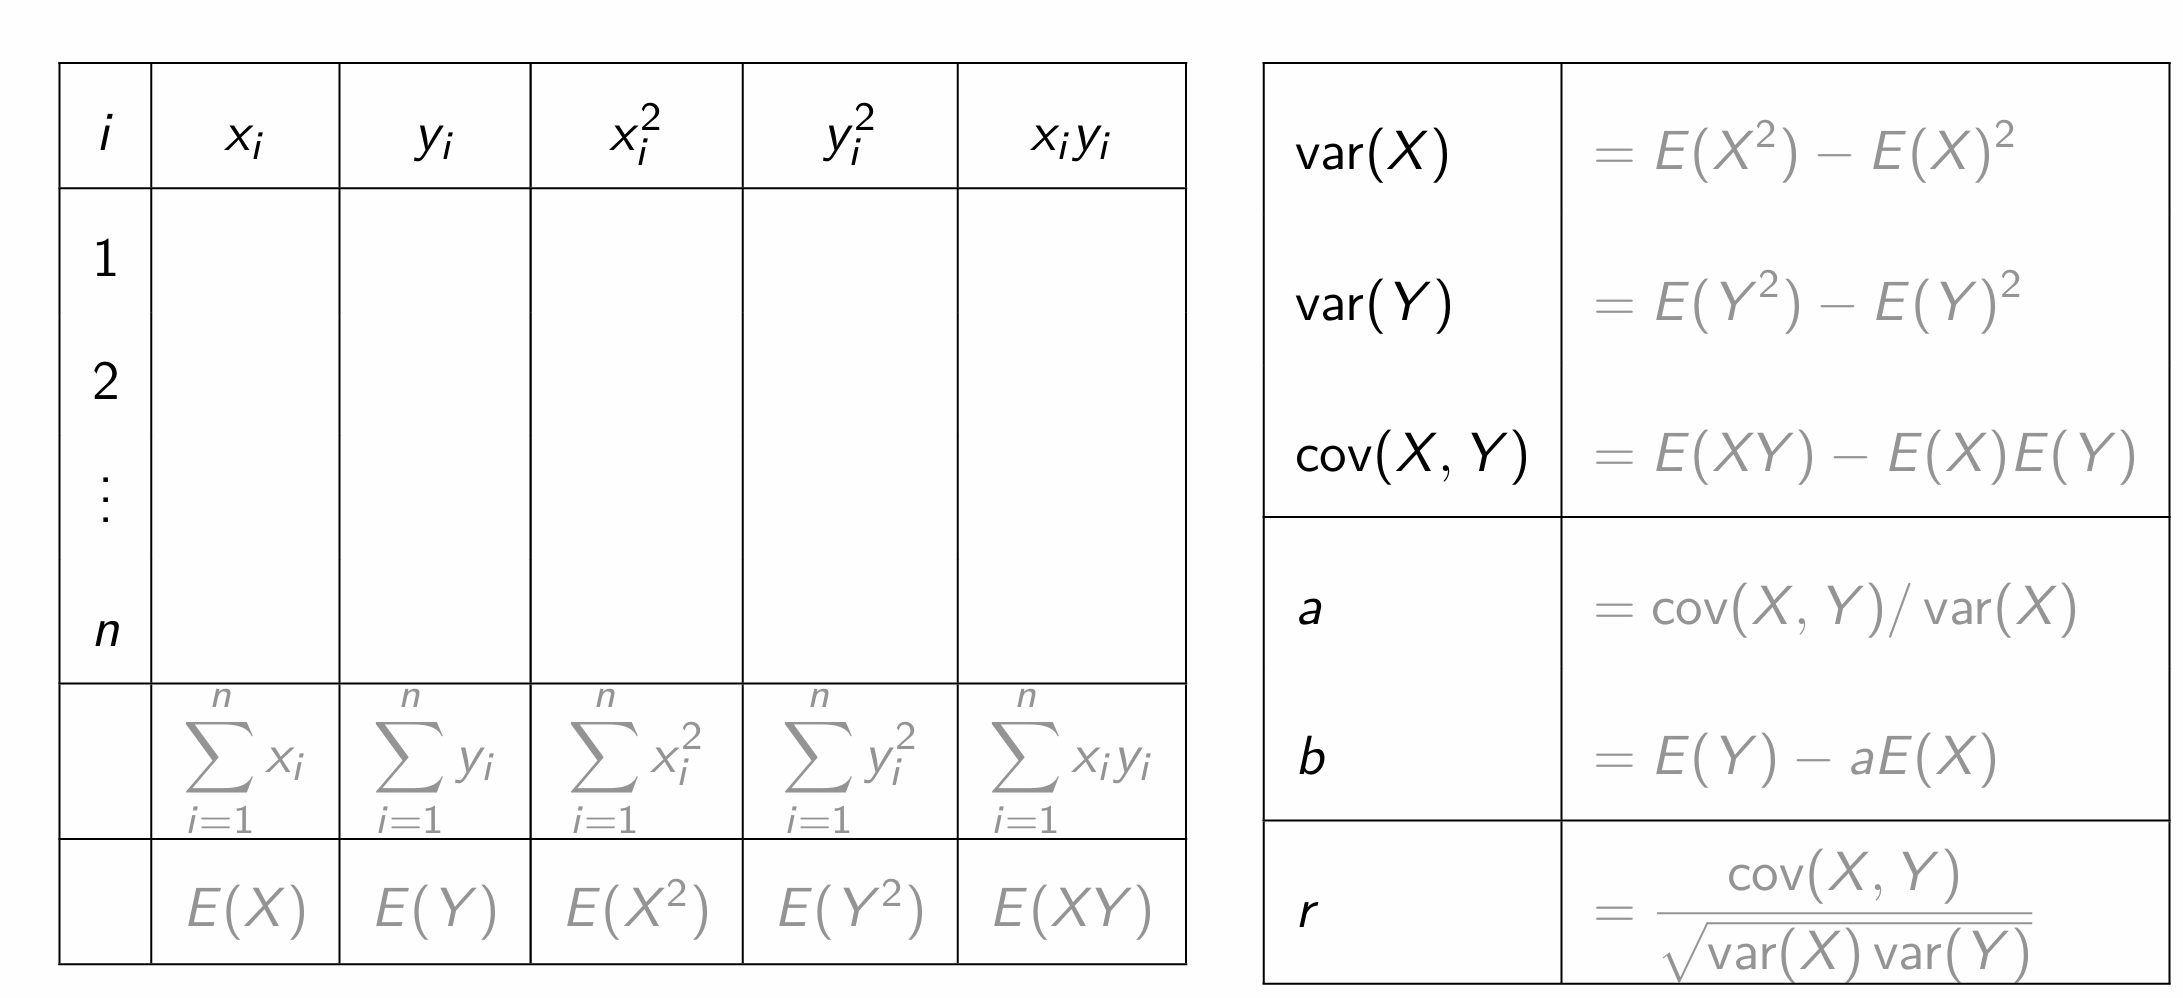
\includegraphics[angle=90,height=1\textwidth]{Images/berechnungsformular-lineare-regression.png}
    \caption{Berechnungsformular für Lineare Regression}
\end{figure}
\newpage

\section{Verteilung}
Bildet das Verständnis für die Lokalisierung von Variabeln.
Es wird hierbei zwischen folgende Typen unterschieden:
\begin{itemize}
    \item quantitativ-diskrete (diskrete Nummer: 1291)
    \item quantitativ-stetig (Skala [20;100])
    \item qualitativ-nominal (Kategorien: Rot, Blau, Pink)
    \item qualitativ-ordinal (Kalt < Warm < Heiss)
\end{itemize}
\defn{Kumulative Häufigkeitsverteilung}{
    Beschreibt die Anzahl Merkmalsausprägungen kleiner als ein 
    bestimmter Schwellenwert.
    \begin{equation}
        H_j = \sum_{k=1}^j h_k = |\{x_i|x_i \leq a_j\}|
    \end{equation}
    Allgemeiner:
    \begin{equation}
        H(x) = |\{ i | x_i \leq x \}|
    \end{equation}
    Die Funktion ist also Stückweise konstant mit Sprungstellen bei \(a_j\),
    und Sprunghöhe \(h_j\).
}
Das Maximum von \(H(x)\) hängt von \(n\) ab, dafür lässt sich
die relative Häufigkeit betrachten:
\begin{equation}
    \begin{split}
        f_j &= \frac{1}{n}h_j \\
        F_j &= \frac{1}{n}H_j \\
        F(x) &= \frac{1}{n}H(x)
    \end{split}
\end{equation}

\defn{Verteilfunktion}{
Die Verteilungsfunktion beschreibt die Wahrscheinlichkeiten der Werte einer Zufallsvariable
\begin{equation}
    F(x)=F_X(x)=P(X\leq x)
\end{equation}
Mit Eigenschaften:
\begin{itemize}
    \item \(F_X(x)\) ist monoton wachsend
    \item \(0 \leq FX(x) \leq 1 \)
    \item \( \lim_{x \to -\infty} = 0 \)
    \item \( \lim_{x \to \infty} = 1 \)
\end{itemize}
Die Verteilfunktion mit \(F(x)\) ist eine Wahrscheinlichkeit
Für ein Intervall gilt: \(P(a < X \leq b)=F_X(b)-F_X(a)\)
}

\begin{figure}[H]
    \centering
    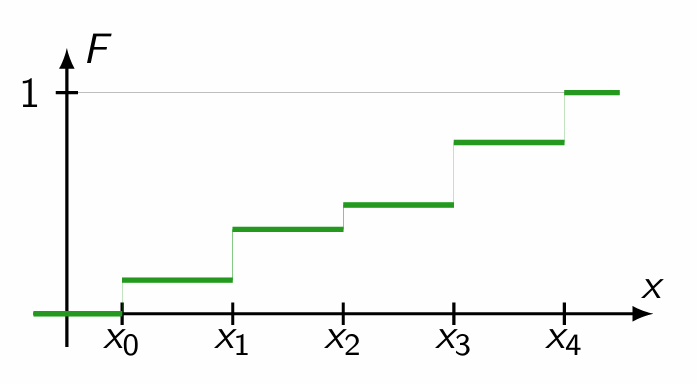
\includegraphics[width=0.5\linewidth]{Images/stetigef.png}
    \caption{Diskrete Verteilfunktion}
\end{figure}
\begin{figure}[H]
    \centering
    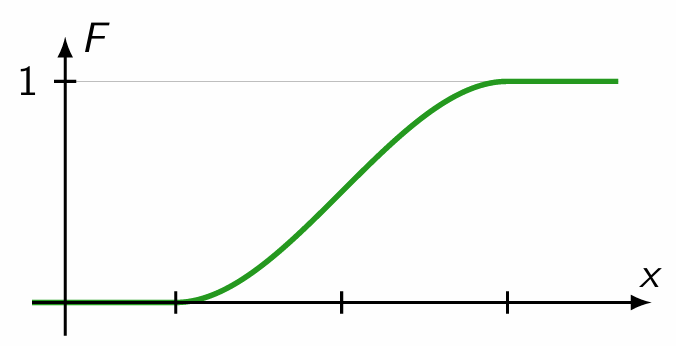
\includegraphics[width=0.5\linewidth]{Images/stetf.png}
    \caption{Stetige Verteilfunktion}
\end{figure}

\subsection{Rezept}
\begin{figure}[H]
    \centering
    \includegraphics[width=0.75\linewidth]{Images/übersicht-verteilung.png}
    \caption{Link Zufallsvariable zu Verteilung}
\end{figure}
\begin{enumerate}
    \item Fragen über \(F(x)\) in Wahrscheinlichkeiten von Ereignissen übersetzen
    \item Rechenregeln für Wahrscheinlichkeiten anwenden
    \item Wahrscheinlichkeiten durch \(F(x)\) ausdrücken, rückübersetzen
\end{enumerate}

\subsection{Verteilfunktion der Max-Funktion}
\defn{Maximum zweier Zufallsvariablen}{
    Für zwei unabhängige Zufallsvariablen \(X,Y\) mit Verteilfunktionen \(F_X(x), F_Y(y)\)
    gilt:
    \begin{equation}
        \begin{split}
            F_{max(X,Y)} &= P(max(X,Y) \leq z) \\
            &= P(X \leq z \land Y \leq z) = P(X \leq z) \cdot P(Y \leq z) \\
            &= F_X(x) \cdot F_Y(y)
        \end{split}
    \end{equation}
}

\begin{figure}[H]
    \centering
    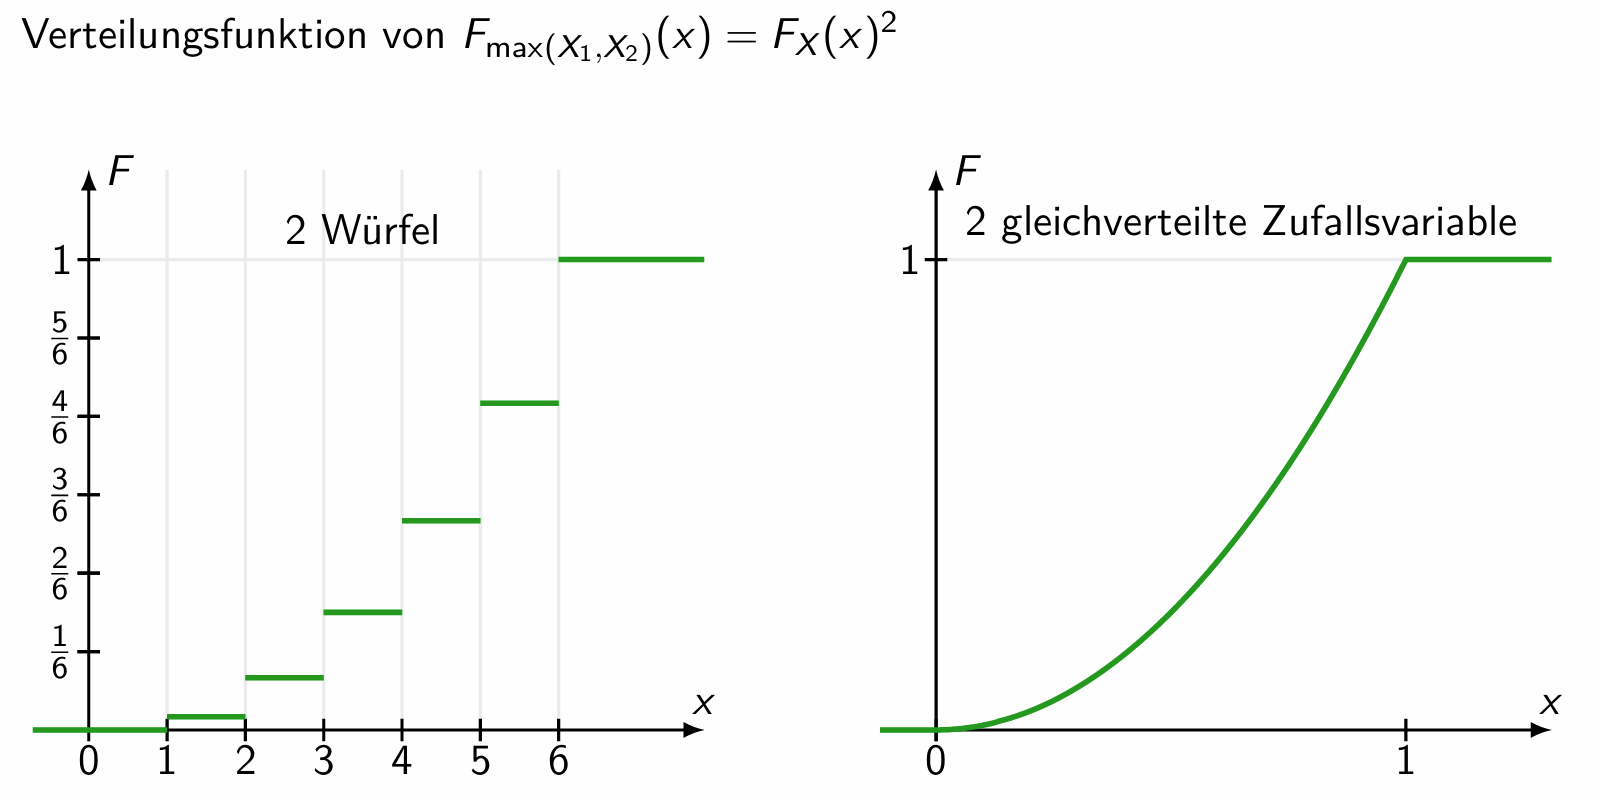
\includegraphics[width=1\linewidth]{Images/verteilung-maximum.png}
    \caption{Verteilung der Max Funktion zweier Variabeln}
\end{figure}

\subsection{Wichtige Punkte}

\begin{figure}[H]
    \centering
    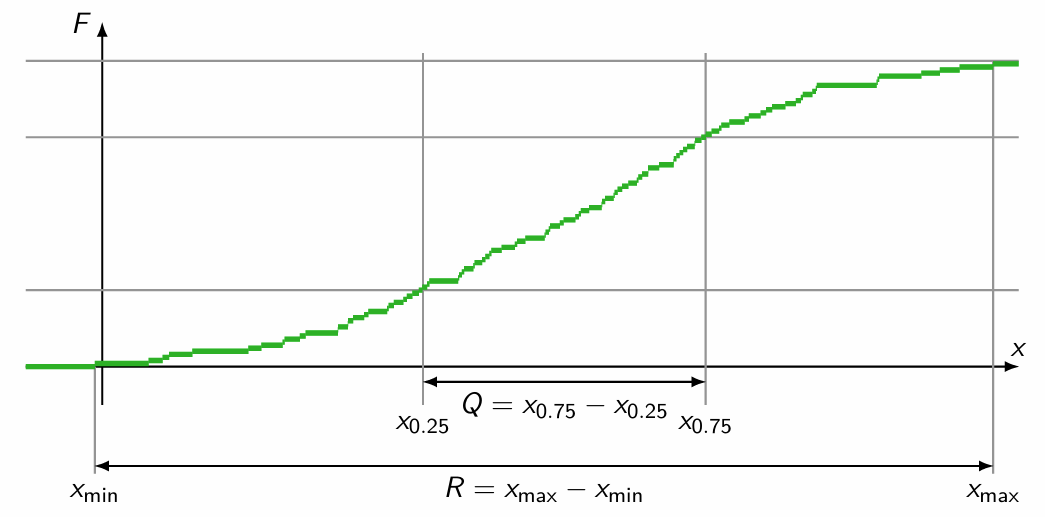
\includegraphics[width=1\linewidth]{Images/spannweitequartilabstand.png}
    \caption{Spannweite R und Quartilabstand Q}
\end{figure}

\defn{Mittelwert}{
    Wir suchen einen Punkt sodass die Momente ausgleichen:
    \begin{equation}
        \bar{x} = \frac{1}{n} \sum x_i
    \end{equation}
    Oder durch dass Minimalprinzip derjenige Punkt in der die Varianz minimiert ist.
    Die Wahrscheinlichkeit einer Abweichung ist dort am kleinsten:
    \begin{equation}
        \text{Minimiert: } \frac{1}{n} \sum (x_i-\bar{x})^2
    \end{equation}
}

\defn{Gewichteter Mittelpunkt}{
    Ist der Punkt an dem die Varianz von gewichteten Punkten minimiert wird.
    Z.B. GPS bei dem die Punkte nicht immer mit der gleichen Genauigkeit berechnet
    werden können.
    \begin{equation}
        \begin{split}
            \bar{x} &= \frac{\sum w_k x_k}{\sum w_k} \\
            \text{Minimiert: } &\sum w_i (x_i - \bar{x})^2
        \end{split}
    \end{equation}
}

\defn{Median}{
    Ist der Punkt in der Mitte (gesehen vom Zahlenstrahl) von vergleichbaren Werten.
    Falls \(n\) gerade ist, ist dies der Mittelwert der beiden mittleren Werte.
    \begin{equation}
        med(x) = x_{0.5} \text{ auch 0.5-Quantil}
    \end{equation}
    Der Wert lässt sich direkt aus \(F_X(x)\) ermitteln:
    \begin{equation}
        F_X(x_{0.5}) = 0.5
    \end{equation}
}

\defn{Quartil}{
    Quartil kann direkt aus \(F_X(x)\) abgelesen werden.
    Sie bezeichnet die Schranken bei für \(P(X \leq x) \leq 0.25\) und \(P(X \leq x) \leq 0.75\).
    \begin{equation}
        F_X(x_{0.\lambda}) = \frac{1}{\lambda}
    \end{equation}

}

\defn{Spannweite}{
    Bezeichnet die Differenz zwischen dem grössten und kleinsten Wert \(R = x_{max} - x_{min}\).
}

\defn{Modus / Modalwert}{
    Der Modus ist der häufigste Wert in einem Datensatz.
}

\subsection{Verteilfunktion und Erwartungswert}
\begin{figure}[H]
    \centering
    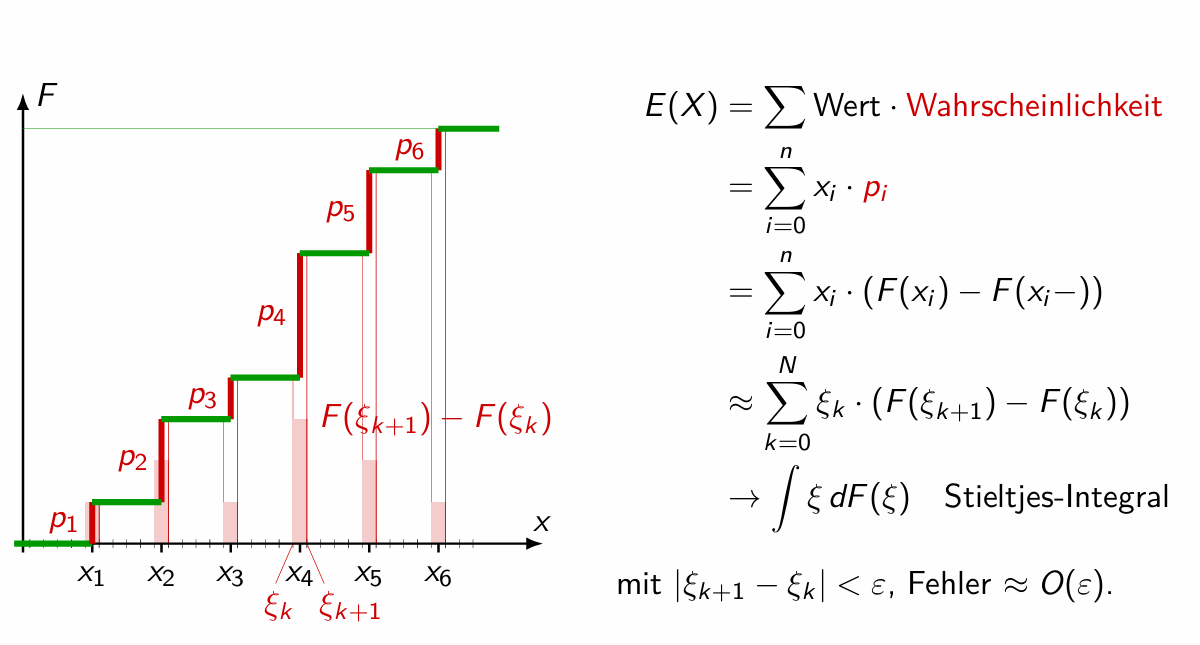
\includegraphics[width=1\linewidth]{Images/verteilungsfunktion-erwartungswert.png}
    \caption{Verteilungsfunktion und Erwartungswert}
\end{figure}

\subsection{Variable gleich verteilen}
Durch erneute Anwendung der Verteilfunktion auf \(X\) wird die Zufallsvariable 
gleichverteilt.
\begin{figure}[H]
    \centering
    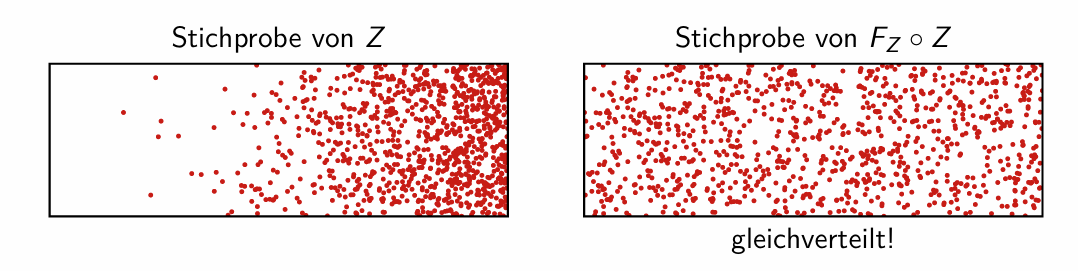
\includegraphics[width=0.75\linewidth]{Images/f_zaufz.png}
    \caption{Erstellung einer Gleichverteilung}
\end{figure}
\textbf{BEISPIEL UND FORMEL!}

\section{Wahrscheinlichkeitsdichte}
\begin{figure}[H]
    \centering
    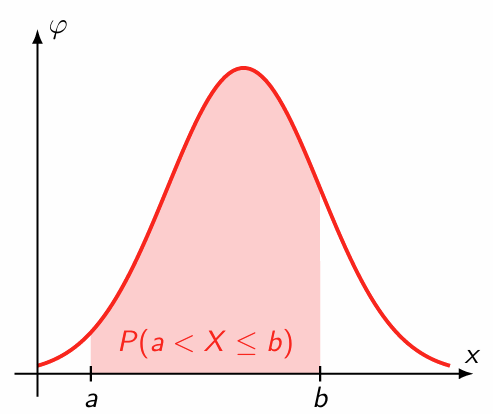
\includegraphics[width=0.5\linewidth]{Images/wahrscheinlichkeitsdichte.png}
    \caption{Wahrscheinlichkeitsdichte}
    \label{fig:enter-label}
\end{figure}
\defn{Wahrscheinlichkeitsdichte Funktion}{
Die Ableitung einer \textbf{stetigen} Verteilungsfunktion heisst
Wahrscheinlichkeitsdichte:
    \begin{equation}
        \varphi(x)=\frac{d}{dx}F(x)=F'(X)
    \end{equation}
    Wenn \(F(x)\) (Verteilfunktion) die Stammfunktion ist bedeutet dies:
    \begin{equation}
        P(a < X \leq b) = \int_a^b \varphi(x) dx
    \end{equation}
}

\subsection{Erwartungswert einer stetigen Verteilung}

\begin{figure}[H]
    \centering
    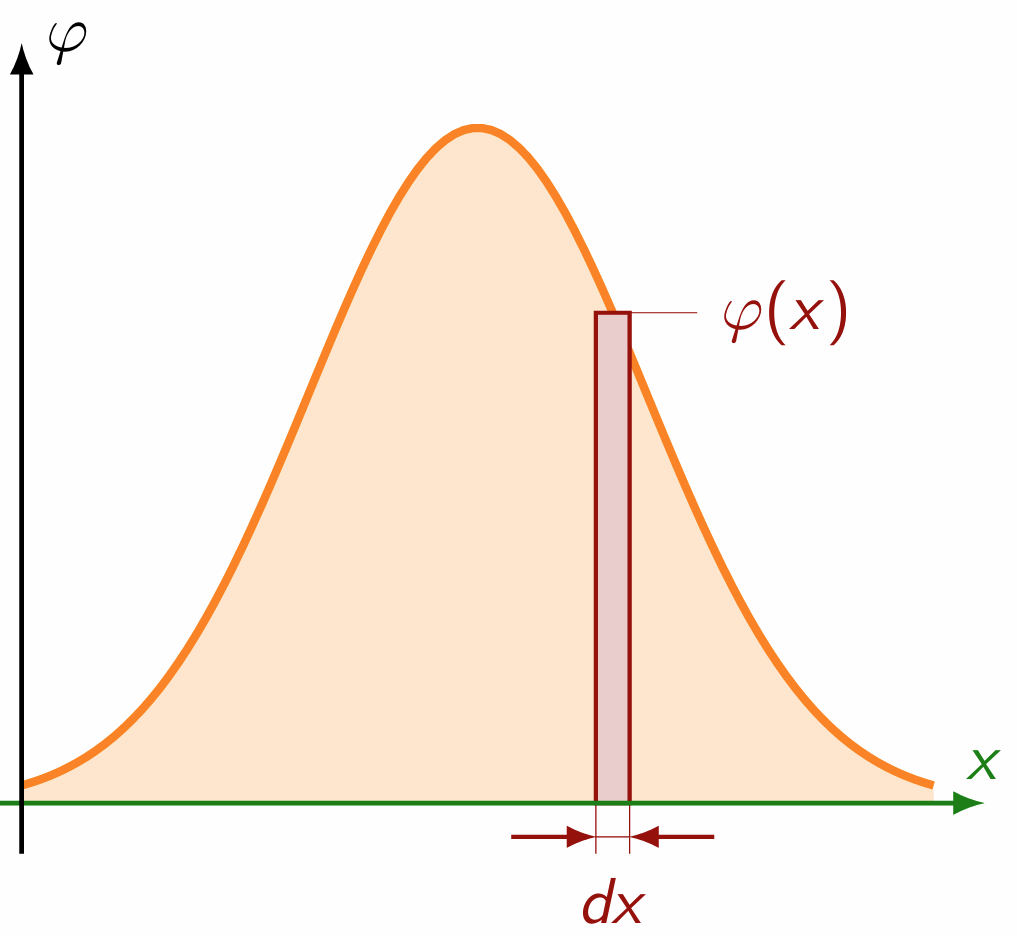
\includegraphics[width=0.5\linewidth]{Images/dichte-erwartungswert.png}
    \caption{Erwartungswert von stetigen Verteilungen}
\end{figure}
\defn{Erwartungswert einer stetigen Verteilung}{
    Mit \(\varphi(x)\), einer Dichtefunktion, kann man nun auch \(E(X)\) berechnen
    einer \textbf{stetigen} Verteilfunktion berechnen:
    \begin{equation}
        \begin{split}
            E(X)&=\sum x \cdot p(x) \\
        & = \int_{-\infty}^\infty x \cdot \varphi(x)dx
        \end{split}
    \end{equation}

    Da der Erwartungswert durch \(\sum \text{Wert }\cdot \text{ Wahrscheinlichkeit}\)
    definiert ist, lässt dieser sich auch über \(\varphi(x)\) berechnen.
    Dabei gilt:
    \begin{equation}
        \begin{split}
            E(X^2) &= \int_{- \infty}^\infty x^2 \varphi dx\\
            E(f(X)) &= \int_{- \infty}^\infty f(x) \varphi dx
        \end{split}
    \end{equation}
}

\subsection{Summe von zwei Zufallsvariablen}
\defn{Summe stetiger Zufallsvariablen (Faltung)}{
    Für beliebige Zufallsvariable \(X\) und \(Y\) gilt mit Dichtefunktion
    \(\varphi_X(x)\) und \(\varphi_Y(y)\) und ihrer Summer \(Z=X+Y\) gilt:
    \begin{equation}
        \varphi_Z(z)=\varphi_{X+Y}(z)=\varphi_X * \varphi_Y(z) = \int_{- \infty}^\infty \varphi_X(x)\varphi_Y(z-x)dx
    \end{equation}
    Für die Verteilsfunktionen gilt:
    \begin{equation}
        F_Z(z)= F_X*\varphi_Y(z)=\varphi_X*F_Y(z)
    \end{equation}
    Dieses Verfahren wird \textbf{Faltung} (eng. Convolution) genannt.
}
\subsubsection{Beispiel}

\begin{figure}[H]
    \centering
    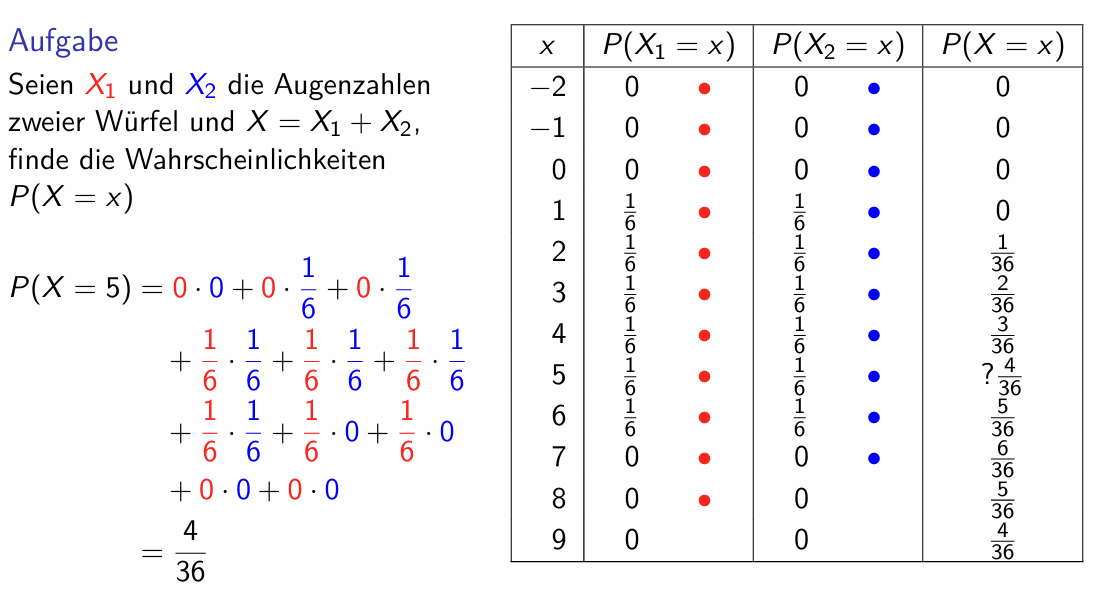
\includegraphics[width=1\linewidth]{Images/faltung-beispiel.png}
    \caption{Beispiel einer Faltung}
\end{figure}

%FALTUNG
\section{Gleichverteilung}

\begin{figure}[H]
    \centering
    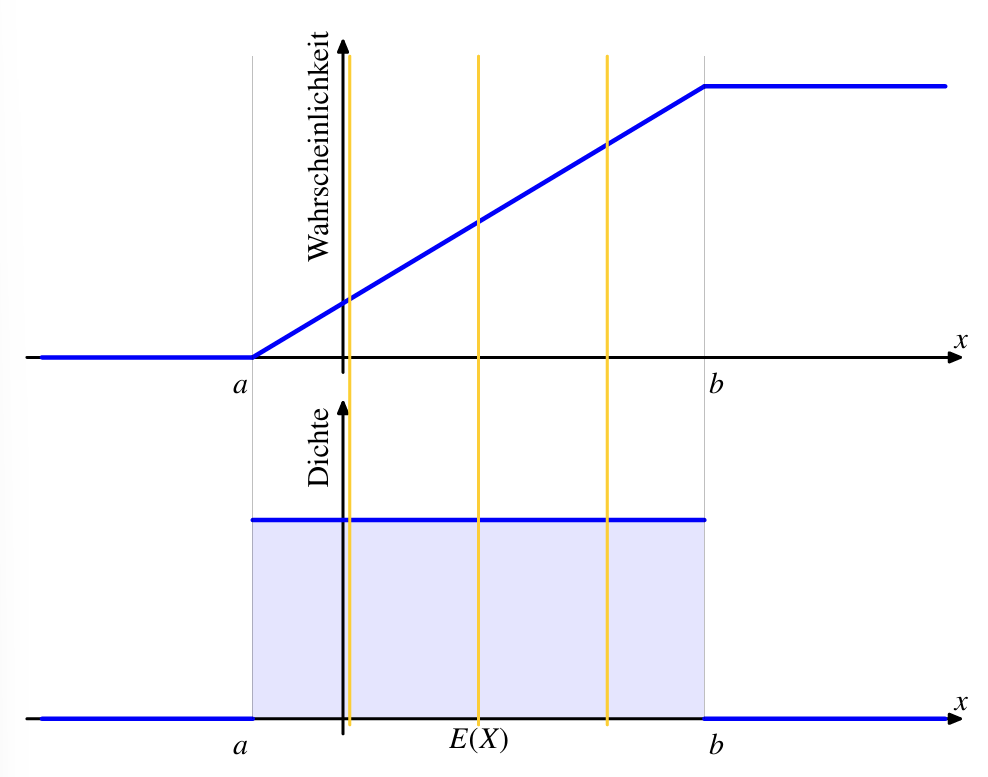
\includegraphics[width=0.75\linewidth]{Images/gleichverteilung.png}
    \caption{Gleichverteilung}
\end{figure}
\defn{Gleichverteilung }{
    \begin{equation}
        \varphi(x)=
        \begin{cases}
            \frac{1}{b-a} &a \leq x \leq b \\
            0 &\text{sonst}
        \end{cases}
    \end{equation}

    \begin{equation}
        F(x) = 
        \begin{cases}
            0  &x \leq a \\
            \frac{x-a}{b-a} &x \leq a \leq b \\
            1 &x > b
        \end{cases}
    \end{equation}
}

\defn{Signifikante Werte}{
    \begin{equation}
        E(X) = \frac{a+b}{2}
    \end{equation}

    \begin{equation}
        \sigma^2 = \frac{(b-a)^2}{12}
    \end{equation}

    \begin{equation}
        x_{\frac{1}{2}}=\frac{a+b}{2}
    \end{equation}
}

\begin{figure}[H]
    \centering
    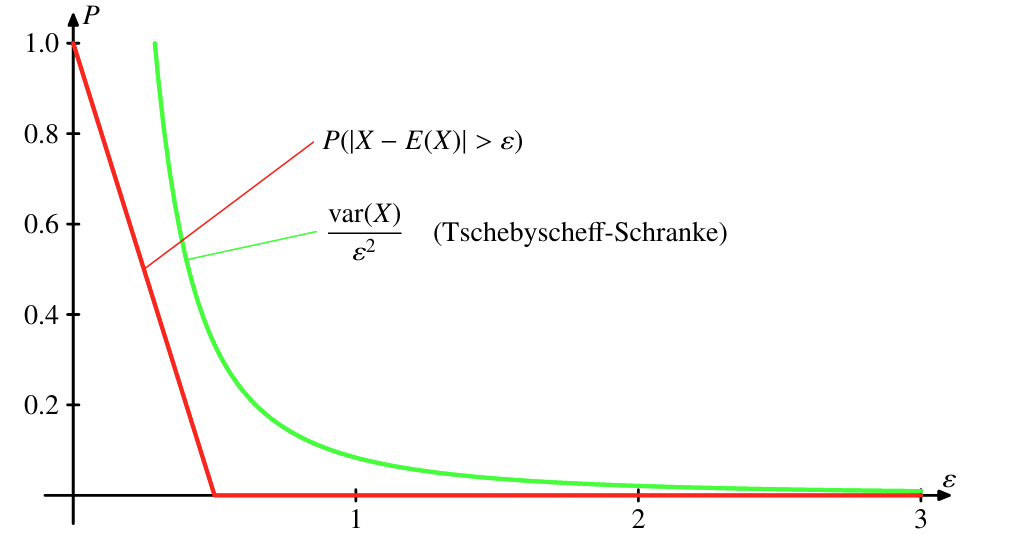
\includegraphics[width=0.75\linewidth]{Images/gleichverteilung-abweichung.png}
    \caption{Abweichung einer Gleichverteilung}
\end{figure}

\defn{Fehlerabschätzung}{
    \begin{equation}
        P(|X-E(X)|>\epsilon)=1\frac{2\epsilon}{b-a} \text{ für } \epsilon < \frac{b-a}{2}
    \end{equation}
}

\subsection{Parameter}

\section{Exponential-Verteilung}
Die positive Zufallsvariable T ist der Zeitpunkt, zu dem ein Ereignis eintritt:
\begin{equation}
    F(x) = P(T \leq x)
\end{equation}
\defn{Gedächtnisloser Prozess}{
    T ist gedächtnislos, wenn die Wahrscheinlichkeit, dass das Ereignis in
    einem Intervall eintrigg, immer gleich ist,
    wenn es zu Beginn des Intervalls noch nicht eingetreten ist:
    \begin{equation}
        P(T \leq y |T>x) = P(T \leq y)
    \end{equation}
}

\exm{Herleitung}{
    \begin{equation}
        \begin{split}
            G(X) &= 1-F(x) \\
            \frac{P(T > x + y)}{P(T>x)} &= P(T > y) \\
            \frac{G(X+y)}{G(X)} &= G(y) \\
            \text{Ableitung nach } y \text{, bei } y&=0 \text{:}\\
            \Rightarrow G'(x) &= G'(0)G(X) \\
            \Rightarrow a &= -G'(0) \\
            \Rightarrow G(x) = Ce^{-ax} &\Rightarrow \varphi(x) = aCe^{-ax}\\
            \Rightarrow \text{für } &x>0\text{, und Normierung: }C=1
        \end{split}
    \end{equation}
}

\defn{Exponential Verteilung }{
    \begin{equation}
        \varphi(x)= ae^{-ax},a>0
    \end{equation}

    \begin{equation}
        F(x) = 1-e^{-ax}
    \end{equation}
}

\begin{figure}[H]
    \centering
    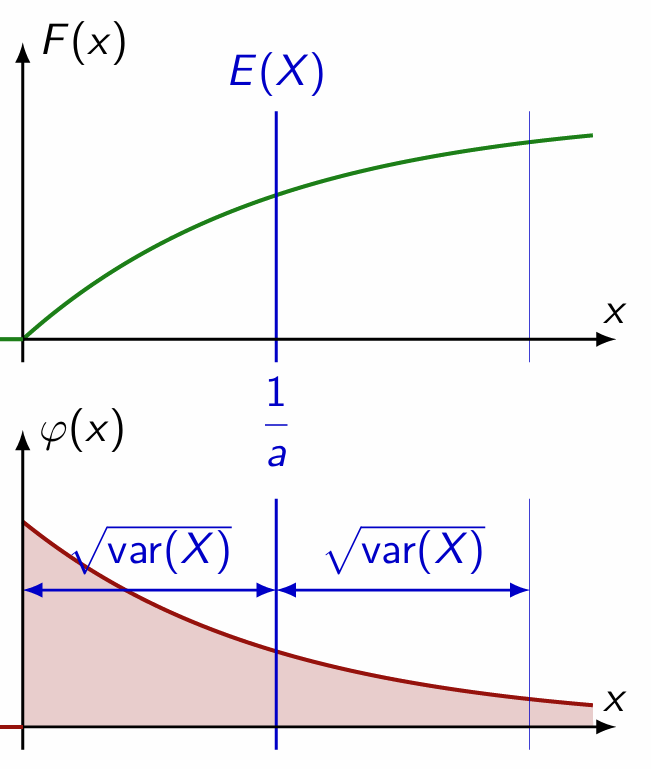
\includegraphics[width=0.5\linewidth]{Images/exp-werte.png}
    \caption{Exponentialverteilung}
\end{figure}

\defn{Signifikante Werte}{
    \begin{equation}
        E(X) = \frac{1}{a}
    \end{equation}

    \begin{equation}
        \sigma^2 = \frac{a}{a^2}
    \end{equation}

    \begin{equation}
        x_{\frac{1}{2}}=\frac{1}{a} log2
    \end{equation}
}

\(\frac{1}{a} = \) Mean Time between Failure.
T bei Median heisst auch Halbwertszeit

\begin{figure}[H]
    \centering
    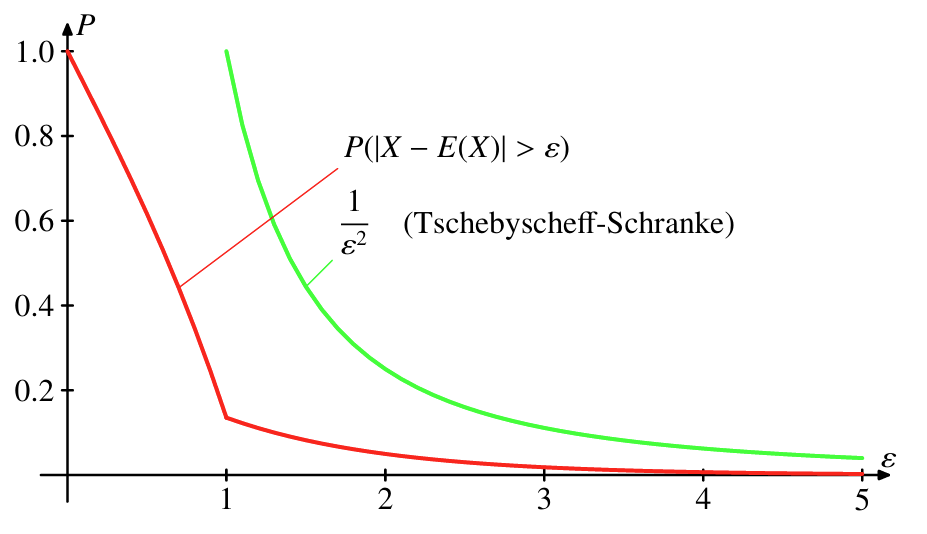
\includegraphics[width=0.75\linewidth]{Images/exp-abweichung.png}
    \caption{Abweichung einer Exponentialverteilung}
\end{figure}

\defn{Fehlerabschätzung}{
    \begin{equation}
        P(|X-E(X)|>\epsilon)=1\frac{2\epsilon}{b-a} \text{ für } \epsilon < \frac{b-a}{2}
    \end{equation}
}

\subsection{Erlang (Summe identischer Exp-Variabeln)}
Für \(X_i\) unabhängige exponentialverteilte
Zufallsvariable mit gleichem Parameter \(a\).
Dann ist \(X_1+\cdots,X_n\) Erlang-verteilt.

\defn{Exponential Verteilung }{
    \begin{equation}
        \varphi(x)= 1-e^{-ax} \sum_{i=0}^{k-1} \frac{(ax)^i}{i!}, x \leq 0
    \end{equation}
    Für \(k =\) Anzahl von Summanden.

    \begin{equation}
        F(x) = a^k \frac{k^{k-1}}{(k-1)!} e{-ax}, x \leq 0
    \end{equation}

    \textbf{Mit \(k=1\) ist die Formel gleicher der Exponentialverteilung.}
}

\begin{figure}[H]
    \centering
    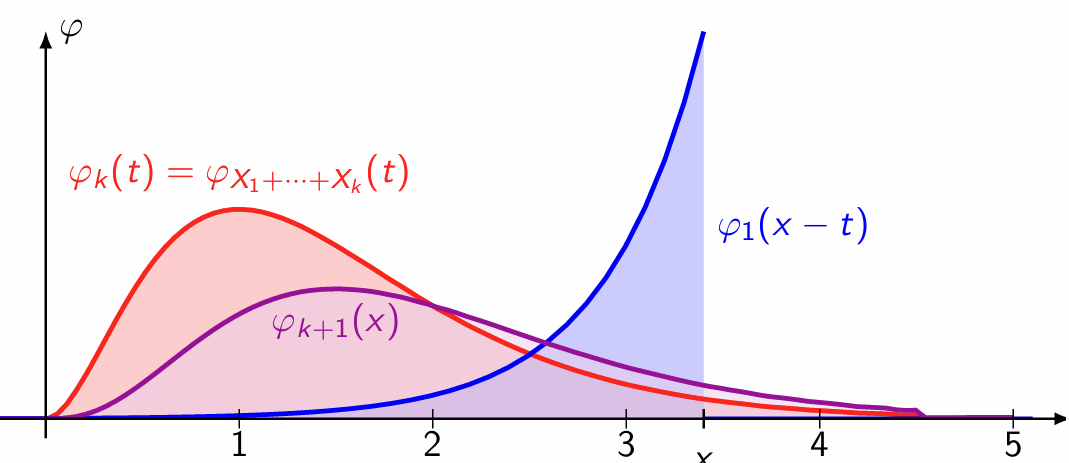
\includegraphics[width=0.75\linewidth]{Images/erlang.png}
    \caption{Erlang Verteilung}
\end{figure}

\subsection{Parameter}

\section{Normalverteilung}
Aufgrund des Zentralen Grenzwertsatzes, welcher besagt,
dass sicher eine Zufallsvariable, welche aus vielen kleinen,
unabhängigigen Zufallseinflüsse besteht, der Normalverteilung
nähert, hat die Normalverteilung eine grosse praktische Bedeutung.

\defn{Normalverteilung}{
    \begin{equation}
        \frac{1}{\sqrt{2\pi\sigma}} e^{-\frac{x-\mu}{2\sigma^2}}
    \end{equation}
}

\begin{figure}[H]
    \centering
    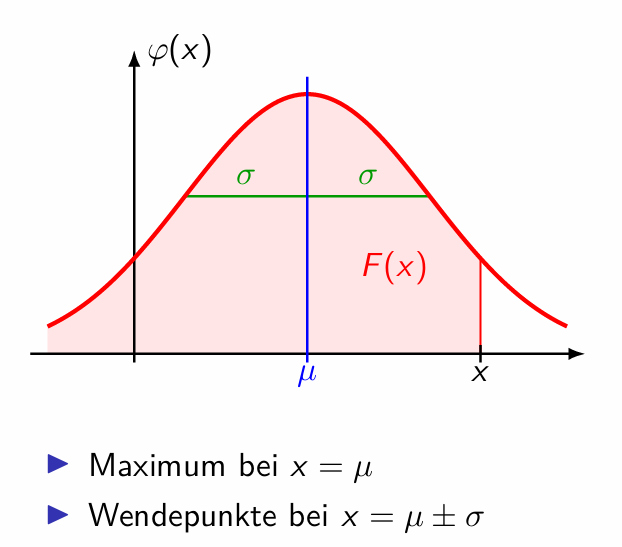
\includegraphics[width=0.5\linewidth]{Images/normalverteilung.png}
    \caption{Normalverteilung}
\end{figure}

\defn{Signifikante Werte}{
    \begin{equation}
        E(X) = \mu
    \end{equation}

    \begin{equation}
        \sigma^2 = \sigma^2
    \end{equation}

    \begin{equation}
        x_{\frac{1}{2}}= \mu
    \end{equation}
}

\begin{figure}[H]
    \centering
    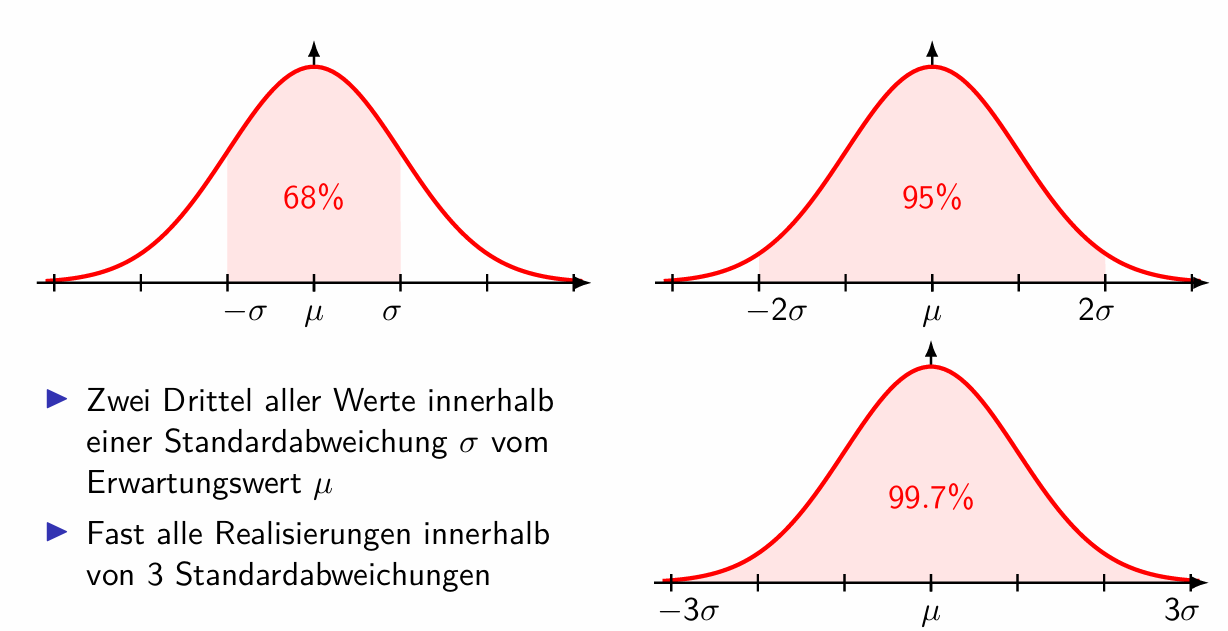
\includegraphics[width=1\linewidth]{Images/norm-typische-werte.png}
    \caption{Typische Werte der Normalverteilung}
\end{figure}

\subsection{Fehlerabschätzung}
Es gibt keine einfache Formel für die Fehlerabschätzung.
Die Verteilungsfunktion der Normalverteilung mit Erwartungswert 0 und Varianz 1,
der sogenannten \textbf{Standardnormalverteilung}, kann nicht in geschlossener Form gefunden werden,
es müssen entweder Tabellen oder numerische  Lösungen verwendet werden.

\subsection{Summe und Linearität}
\defn{Linearität}{
    Ist \(X\) normalverteilt, dann gilt:
    \begin{equation}
        aX+b = \text{ normalverteilt}
    \end{equation}
}

\defn{Summensatz}{
    Die Summe zweier unabhängigeger Zufallsgrössen sind wieder normalverteilt.

    Sind \(X_1, X_2\) normalverteilte Zufallsgrössen mit Mittelwert \(\mu_x\),
    und Varianz \(\sigma_x\), dann ist  \(X_1+X_2\) ebenfalls normalverteilt mit
    \(\mu = \mu_1+\mu_2\) und \(\sigma^2 = \sigma_1^2+\sigma_2^2\).
}

\subsection{Fehlerabschätzung}

\begin{figure}[H]
    \centering
    \includegraphics[width=1\linewidth]{Images/fehlerabschätzung-norm.png}
    \caption{Fehlerabschätzung der Normalverteilung}
\end{figure}

\subsection{Zentraler Grenzwertsatz}
\defn{Zentraler Grenzwertsatz}{
    Sind \(X_1,X_2,\dots\) identisch verteilte und unabhängige Zufallsvariabeln mit \(E(X_i)=\mu\)
    und \(var(X_i)=\sigma^2\), dann gilt:
    \begin{equation}
        S_n = \sum_{i=1}^{n} X_i \Rightarrow E(S_n) = n\mu, var(S_n) = n\sigma^2
    \end{equation}
    Und somit für das neue \(Z\):
    \begin{equation}
        Z_n = \frac{S_n-n\mu}{\sqrt{n}\sigma} \Rightarrow E(Z_n) = 0, var(Z_n) = 1
    \end{equation}

    Für \(n \to \infty\) strebt die Verteilung von \(Z_n\) gegen die Standardnormalverteilung, d.h:
    \begin{equation}
        \lim_{n \to \infty} P(Z_n \leq z) = \phi(z)
    \end{equation}    

    Die Summe vieler vergleichbarer kleiner Einflüssse ist annähernd normalverteilt.
}

\begin{figure}[H]
    \centering
    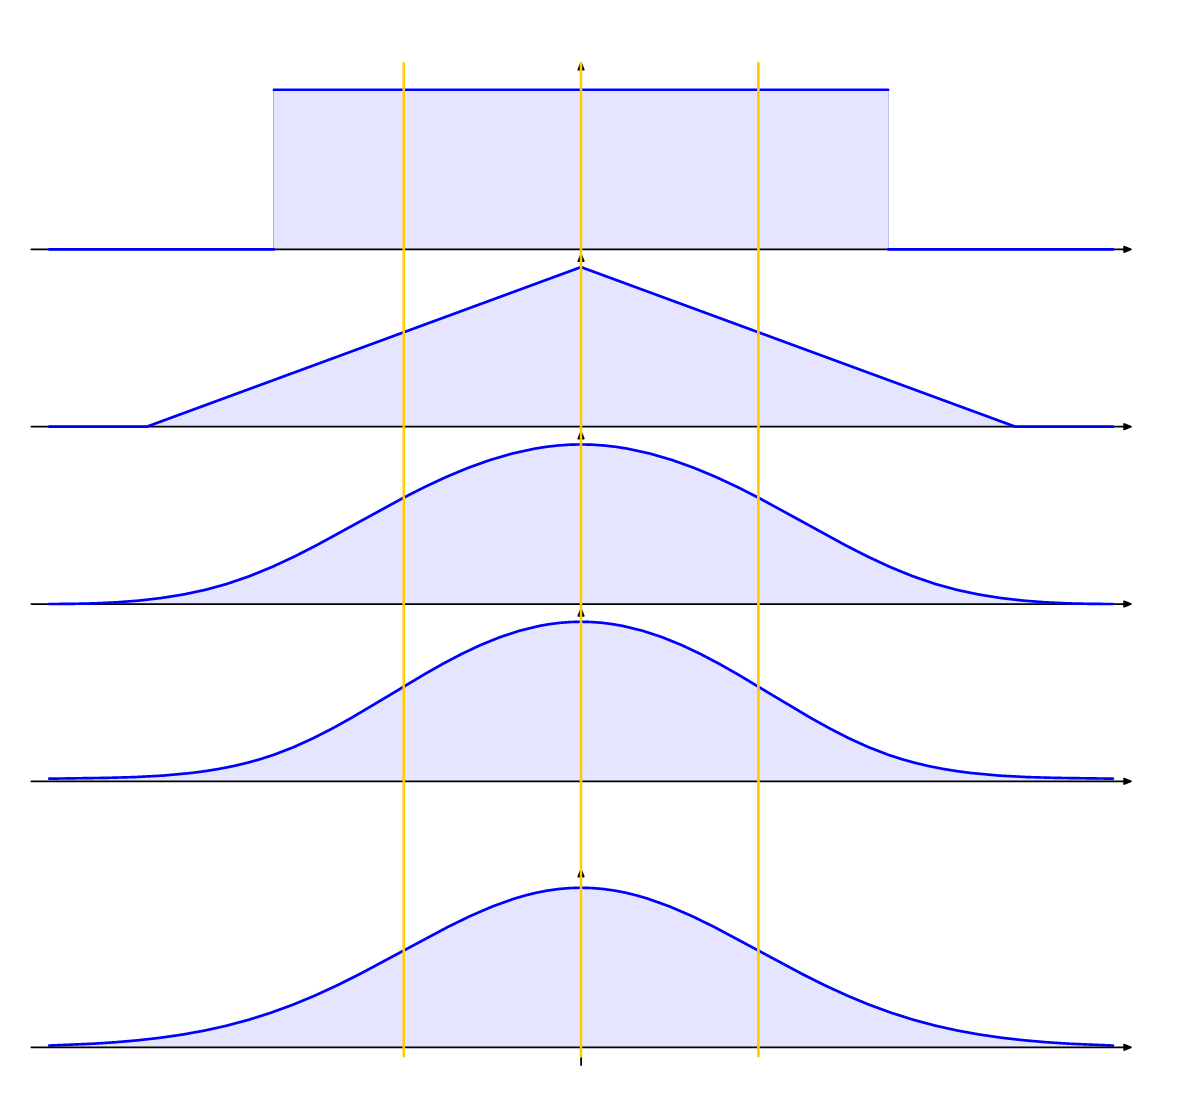
\includegraphics[width=0.75\linewidth]{Images/central-limit.png}
    \caption{Zum zentralen Grenzwertsatz: Die Wahrscheinlichkeitsdichte der standardisierten Summe von
    bis zu vier gleichverteilten Zufallsvariablen (oben) konvergiert gegen die Standardnormalverteilung (unten)}
\end{figure}

\defn{Faltungseigenschaft}{
    Für \(\varphi_i\) eine Normalverteilungsdichte mit \(\mu_i\) und \(\sigma_i\), dann ist
    \(\varphi_1 * \varphi_2\) eine Normalverteilungsdichte mit \(\mu = \mu_1 + \mu_2\) und
    \(\sigma^2 = \sigma_1^2 + \sigma_2^2\).
}

\defn{Summe}{
    Sind \(X_i\) Zufallsvariabeln mit \(E(X_i) = 0\) und \(var(X_i) = 1\), dann konvergiert die
    Verteilungsfunktion von:
    \begin{equation}
         S_n = \frac{X_1+\dots+ X_n}{\sqrt{n}}
    \end{equation}
    Gegen eine Normalverteilung mit \(\mu = 0 \) und \(\sigma = 1\)
}

\subsection{Standardnormalverteilung}
Die Standardnormalverteilung ist die Verteilung mit \(E(X)=0\) und
\(\sigma^2 = 1\).

Eine beliebige Standardverteilte Variabel kann in diese Form gebracht werden:
\begin{equation}
    Z = \frac{x-\mu}{\sigma}
\end{equation}

\defn{Standardnormalverteilung}{
    Ist \(Z = \frac{x-\mu}{\sigma}\), dann ist \(Z\) standard normalverteilt,
    mit \(E(Z)=0\) und \(var(Z)=1\). \(Z\) heisst \textbf{Standardnormalverteilung},
    mit Verteilungsfunktion \(\phi(z)\).

    Es gilt:
    \begin{equation}
        \phi(-z) = 1 -\phi(z)
    \end{equation}
}

\subsection{Normnalverteilungstabelle}

\begin{figure}[H]
    \centering
    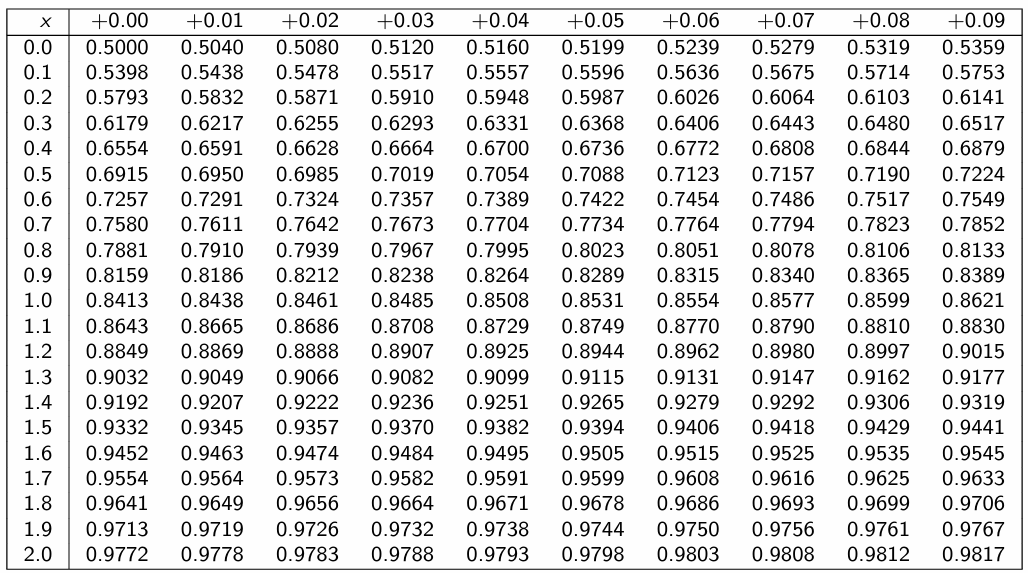
\includegraphics[width=1\linewidth]{Images/norm-tabelle.png}
    \caption{Verteilungsfunktion der Normalverteilung}
\end{figure}
\begin{figure}[H]
    \centering
    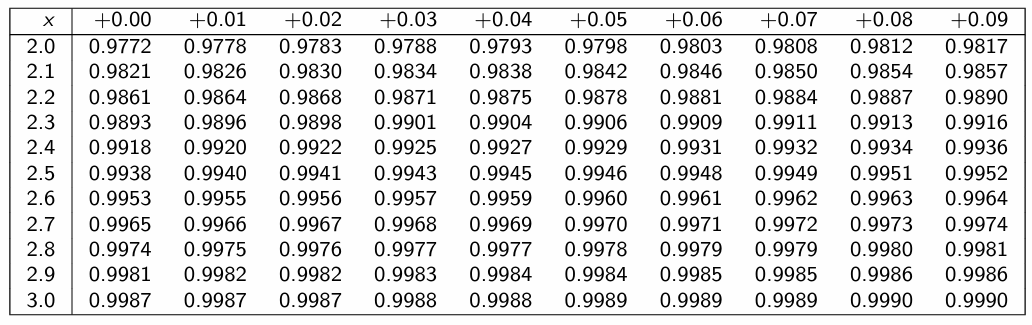
\includegraphics[width=1\linewidth]{Images/norm-tabelle-2.png}
    \caption{Verteilungsfunktion der Normalverteilung 2}
\end{figure}

\subsection{ADD KENDALL NOTATION}

\section{Binomial-Verteilung}
Die Binomialverteilung modelliert Zufallsexperimente mit zwei möglichen Ausgängen \(A\) oder \(\bar{A}\).
 \defn{Binomial Verteilung }{
    Dabei ist \(X\) die Anzahl der eingetrettenen \(A\) in \(n\) unabghängigen Durchführungen.

    \begin{equation}
        P(X=k) = \binom{n}{k} p^k (1-p)^{n-k}
    \end{equation}

    \begin{equation}
        F(x) = 1-e^{-ax}
    \end{equation}
}

\begin{figure}[H]
    \centering
    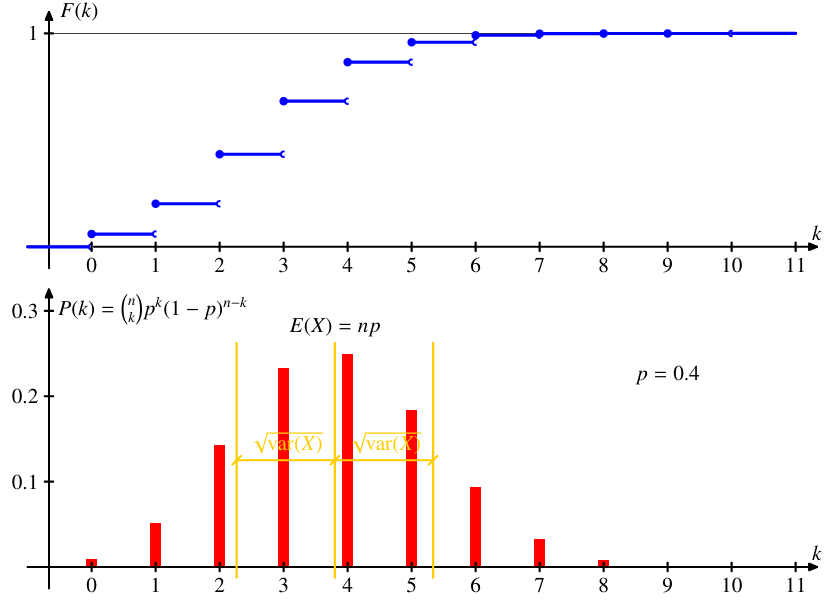
\includegraphics[width=0.75\linewidth]{Images/binomial-verteilung.png}
    \caption{Binomialverteilung}
\end{figure}

\defn{Wichtige Kennzahlen}{
    \begin{equation}
        \begin{split}
            E(X) &= np \\
            var(X) &= np(1-p)
        \end{split}
    \end{equation}
    Wenn \(X\) die Summe von \(n\) 0-1-Einflüssen ist, dann ist
    diese approximativ normalverteilt mit \(\mu = np \) und \(\sigma^2 = np(1-p)\).
}

\subsection{Berechnungsprobleme}

\begin{figure}[H]
    \centering
    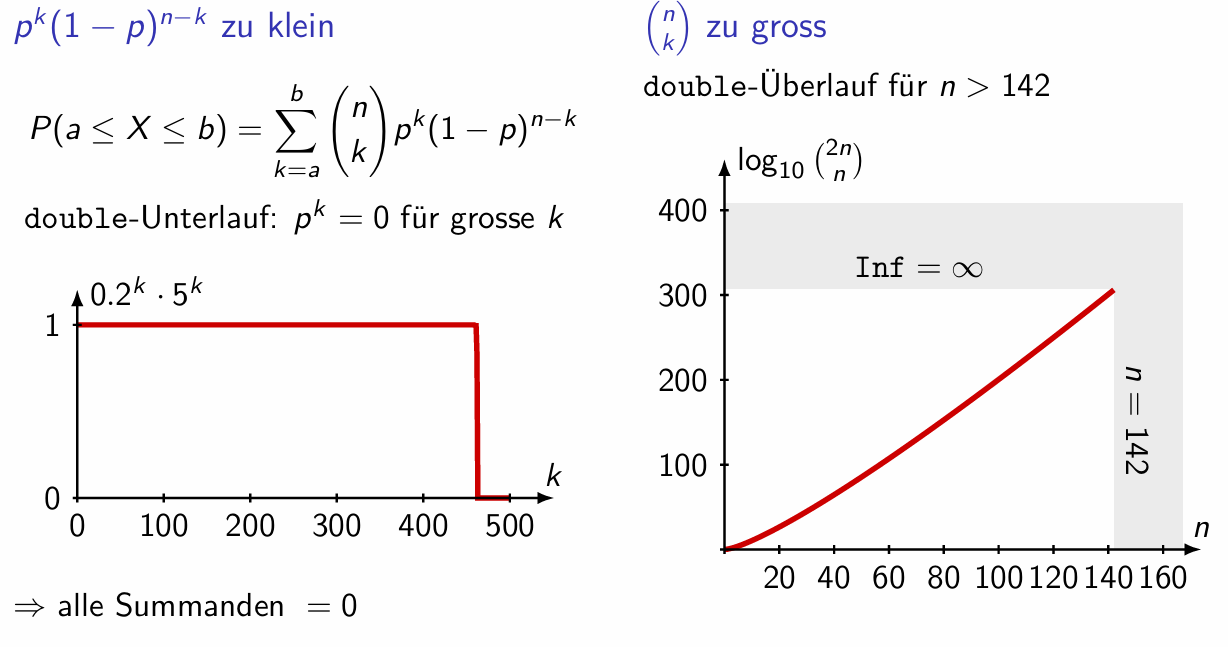
\includegraphics[width=0.75\linewidth]{Images/binom-berechnungsprobleme.png}
    \caption{Berechnungsprobleme der Binomialverteilung}
\end{figure}

\subsection{Normalapproximation}

\begin{figure}[H]
    \centering
    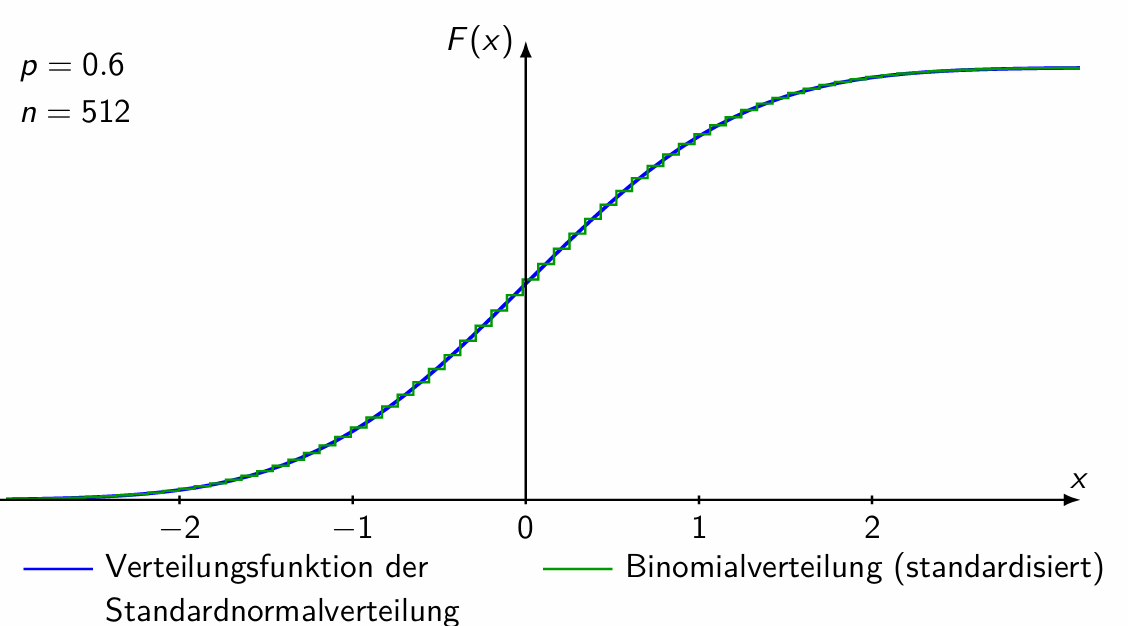
\includegraphics[width=0.75\linewidth]{Images/normalapproximation.png}
    \caption{Normalapproximation}
\end{figure}

Bei gegebener Binomialverteilung \(X\) lässt sich diese approximativ normalverteilt behandeln mit
\(\mu = np\) und \(sigma^2 = np (1-p)\), daraus lässt sich folgendes bilden:
\defn{Normalapproximation}{
    \begin{equation}
        Z =  \frac{X-\mu}{\sigma} = \frac{X-np}{\sqrt{np(1-p)}}
    \end{equation}
}

Damit lässt sich einfacher rechnen:
\begin{equation}
    P(a < X \leq b) = \phi(\frac{b-np}{\sqrt{np(1-p)}}) - \phi(\frac{a-np}{\sqrt{np(1-p)}})
\end{equation}
Für eine genauere Approximation, kann folgendes benutzt werden:
\begin{equation}
    P(a < X \leq b) = \phi(\frac{b+0.5-np}{\sqrt{np(1-p)}}) - \phi(\frac{a+0.5-np}{\sqrt{np(1-p)}})
\end{equation}

\subsection{TODO Approximation für seltene Ereignisse}
POISSON BENUTZEN!!

\section{TODO: Hypergeometrische Verteilung}
Die hypergeometrische Verteilung wird benutzt um
diskrete Wahrscheinlichkeiten eines Auswahlproblems zu bestimmen.

Im üblichen Fall wird dabei von \(N\) Objekten \(M\) markiert.
Daraus werden \(n\) Objekte zufällig ausgewählt.

\defn{Hypergeometrische Verteilung}{
    \begin{equation}
        P(X=m) = \frac{\binom{M}{m}\binom{N-M}{n-m}}{\binom{N}{n}}
    \end{equation}
}

\defn{Wichtige Eckpunkte}{
    \begin{equation}
        \begin{split}
            E(X) &= n\frac{M}{N} \\
            var(X) &= n\frac{M}{N}(1-\frac{M}{N})\frac{N-n}{N-1}
        \end{split}
    \end{equation}
}

\subsection{Begründung für hg Verteilung}
    
\begin{figure}[H]
    \centering
    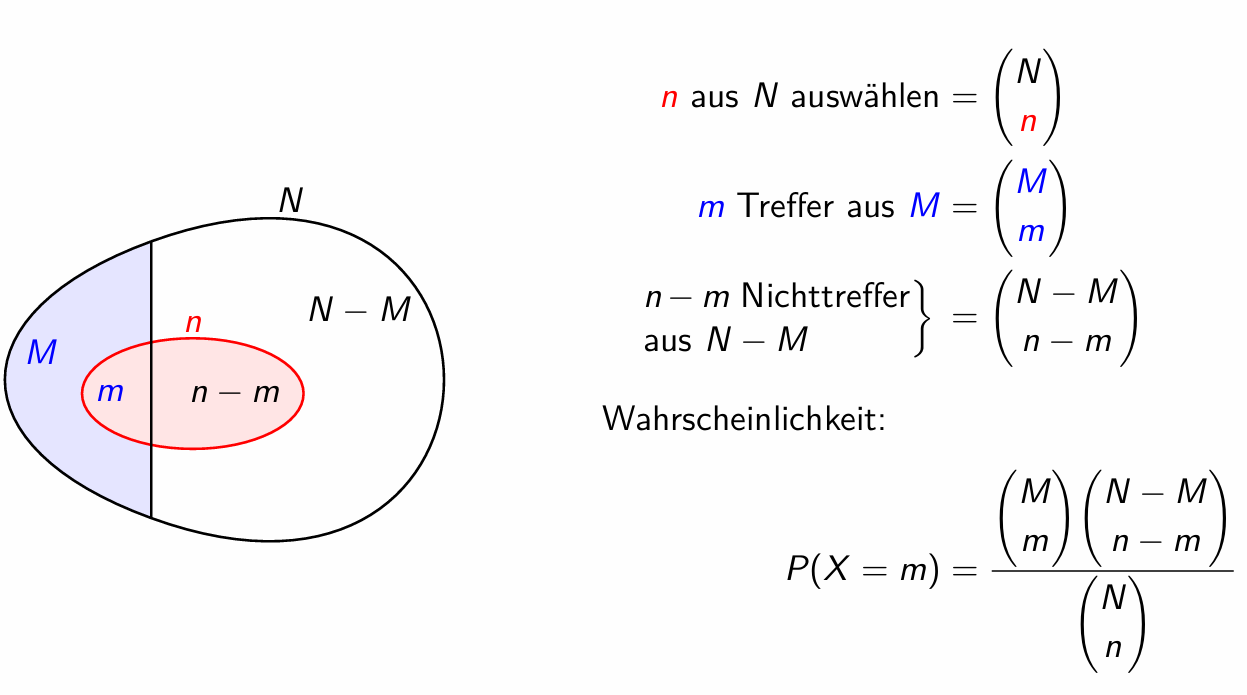
\includegraphics[width=0.75\linewidth]{Images/begr-hg-verteilung.png}
    \caption{Begründung der hypergeometrischen Verteilung}
\end{figure}

\section{Poisson-Verteilung}
\section{Potenzverteilung}
Für Skaleninvatiante Prozesse:
\begin{equation}
    \varphi(bx) = g(b)\varphi(x)
\end{equation}
Das heisst mit der Skalierung von \(x\) mit \(b\) ändert sich
an der Form von \(\varphi\) nichts für \(x > x_{min}\).
Der Faktor \(g(b)\) heisst Renormierung.

\defn{Potenzverteilung}{
    \begin{equation}
        \varphi(x) = \frac{\alpha - 1}{x_{min}}(\frac{x}{x_{min}})^{-\alpha}, \text{für } x\leq x_{min}
    \end{equation}
    \begin{equation}
        F(x) = 1- (\frac{x}{x_{min}})^{1- \alpha} \text{für } x\leq x_{min}
    \end{equation}
}

Um eine Rangfunktion zu erhalten rechnet man:
\begin{equation}
    \text{Rangfunktion} = log(1-F(X))
\end{equation}
Ergibt eine Art Rangfolge der Verteilung.

\begin{figure}[H]
    \centering
    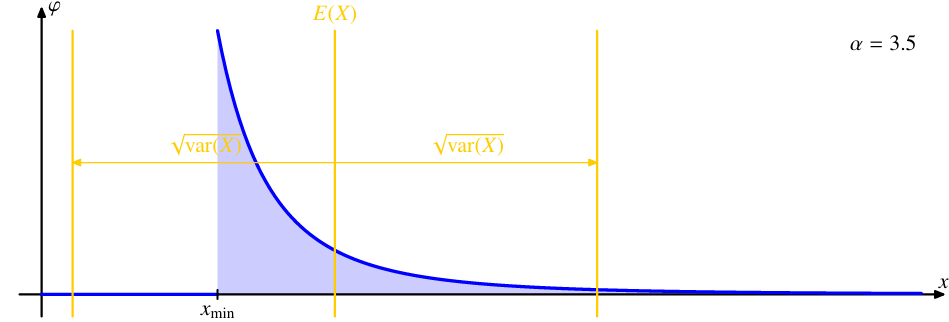
\includegraphics[width=1\linewidth]{Images/potenzverteilung.png}
    \caption{Potenzverteilung}
\end{figure}

\begin{figure}[H]
    \centering
    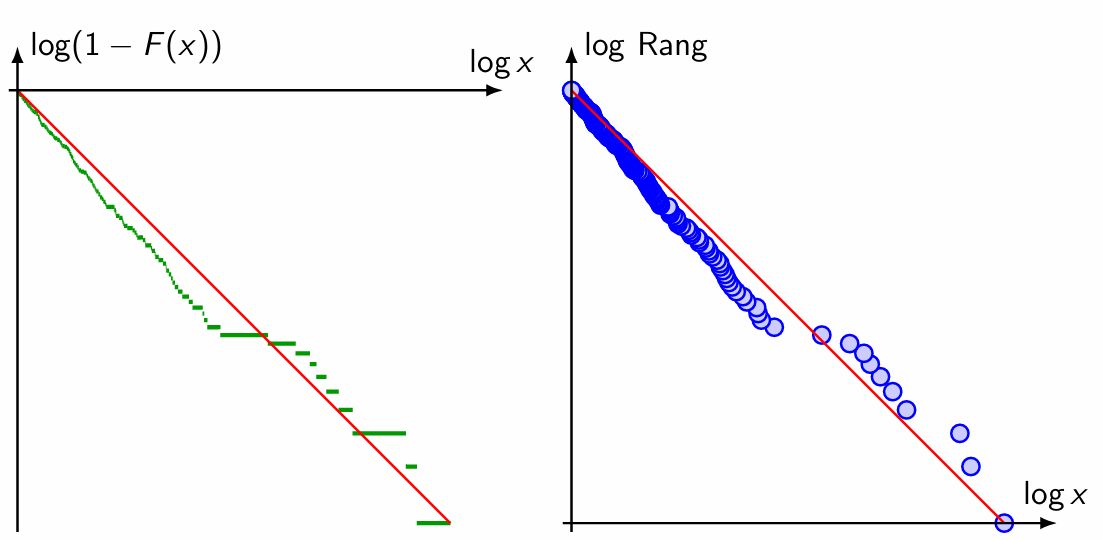
\includegraphics[width=0.75\linewidth]{Images/potenz-verteilfunktion-rang.png}
    \caption{Potenzverteilung Verteilfunktion und Rang}
\end{figure}

\subsection{Wichtige Kennzahlen}
\defn{Kennzahlen}{
    \begin{equation}
        \begin{split}
            med(X) &= 2 \frac{1}{\alpha -1} x_{min} \\
            E(X) &= \frac{\alpha - 1}{\alpha - 2} x_{min} \\
            var(X) &= ( \frac{\alpha - 1}{\alpha - 3} - (\frac{\alpha - 1}{\alpha - 2}^2)) x_{min}^2
        \end{split}
    \end{equation}
    Für E(X) und var(X) gilt für Werte \(\alpha \leq 2\) und \(\alpha \leq 3\) macht die Bezeichnung keinen Sinn.
    Daher ist oft nur der Median angegeben.
}

\subsection{Zipfs Law}

\begin{figure}[H]
    \centering
    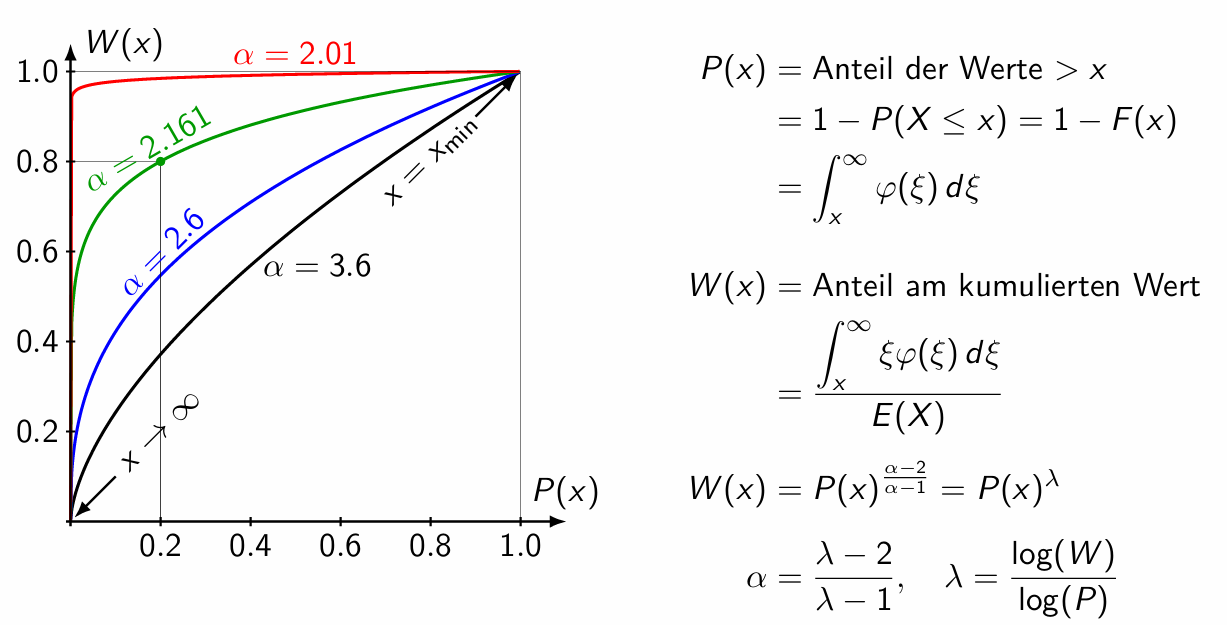
\includegraphics[width=0.75\linewidth]{Images/80-20.png}
    \caption{80/20-Regel}
\end{figure}
Man kann W(x) als den Anteil des "Wertes" interpretieren, den die Werte oberhalb von x bei
steuern. Es ist klar, dass P(x) = 1 auch bedeutet, W(x) = 1: 100\% der Werte tragen 100\% des
 Wertes bei. Die Definitionen besagen, dass für beliebiges x der obere P(x)-Anteil der Werte den
 Anteil W(x) des gesamten Wertes beitragen.

 \exm{80/20-Regel}{
    Gesucht ist z.B. \(\alpha\) für eine Einkommensverteilung,
    bei der die top 1\% 40\% des Vermögens besitzen:
    \begin{equation*}
        \begin{split}
            \lambda &= \frac{log 0.4}{log 0.01} \\
            \alpha &= \frac{\lambda-2}{\lambda-1} = 2.2484
        \end{split}
    \end{equation*}

 }

\section{Schätzprobleme}
Ein Schätzproblem ist eine Aufgabe, bei der die Parameter \(\vartheta\) einer gegebenen
Verteilung gefunden werden sollen. Gegeben ist also \(X\) mit Verteilung
\(\varphi(x,\vartheta)\) und \(x_1,\dots,x_n\) Beobachtungen.
Gesucht ist eine möglichst gute Schätzung für: \(\hat{\vartheta}(x_1,\dots,x_n)\).
Desweiteren möchten wir wissen, wie die Schätzwerte verteilt sind mit
Stichproben \(X_i,\dots,X_n\):
\begin{equation}
    \hat{\vartheta} = \hat{\vartheta}(X_i,\dots,X_n)
\end{equation}

\defn{Stichprobe}{
    Eine Folge von Zufallsvariabeln \(X_i\) heisst eine Stichprobe der Zufallsvariabeln \(X\),
    wenn \(X_i\) unabhängige und identisch zu \(X\) verteilt sind.
}

\defn{Konsistent}{
    Ein Schätzer ist konsistent, wenn dieser korrekt ist für genügend
    grosse Stichproben:
    \begin{equation}
        \lim_{n \to \infty} \hat{\vartheta}(x_i,\dots,x_n)= \vartheta
    \end{equation}
}

\defn{Erwartungstreu}{
    Ein Schätzer ist erwartungstreu, wenn dieser korrekt ist selbst für
    kleine Stichproben:
    \begin{equation}
        E(\hat{\vartheta}(X_1,\dots,X_n))= \vartheta
    \end{equation}
}

\begin{figure}[H]
    \centering
    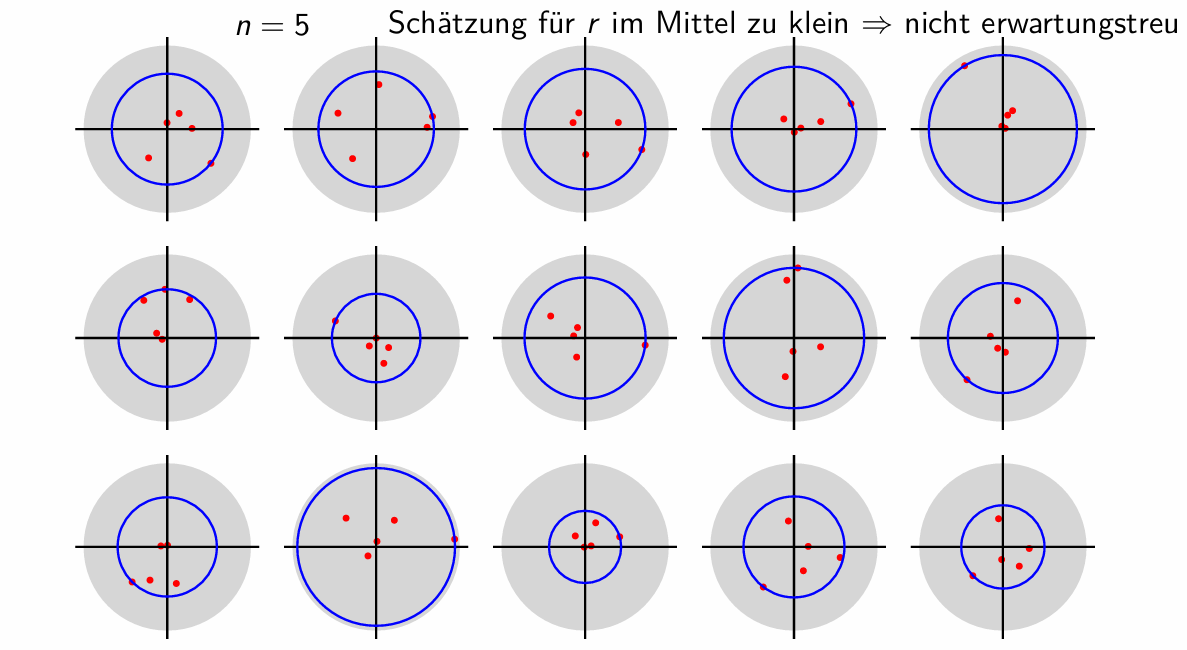
\includegraphics[width=1\linewidth]{Images/beispiel-nichterwartungstreu-radius.png}
    \caption{Beispiel einer nicht erwartungstreuen Schätzung des Radius}
\end{figure}

\subsection{Maximum-Likelihood}
\begin{figure}[H]
    \centering
    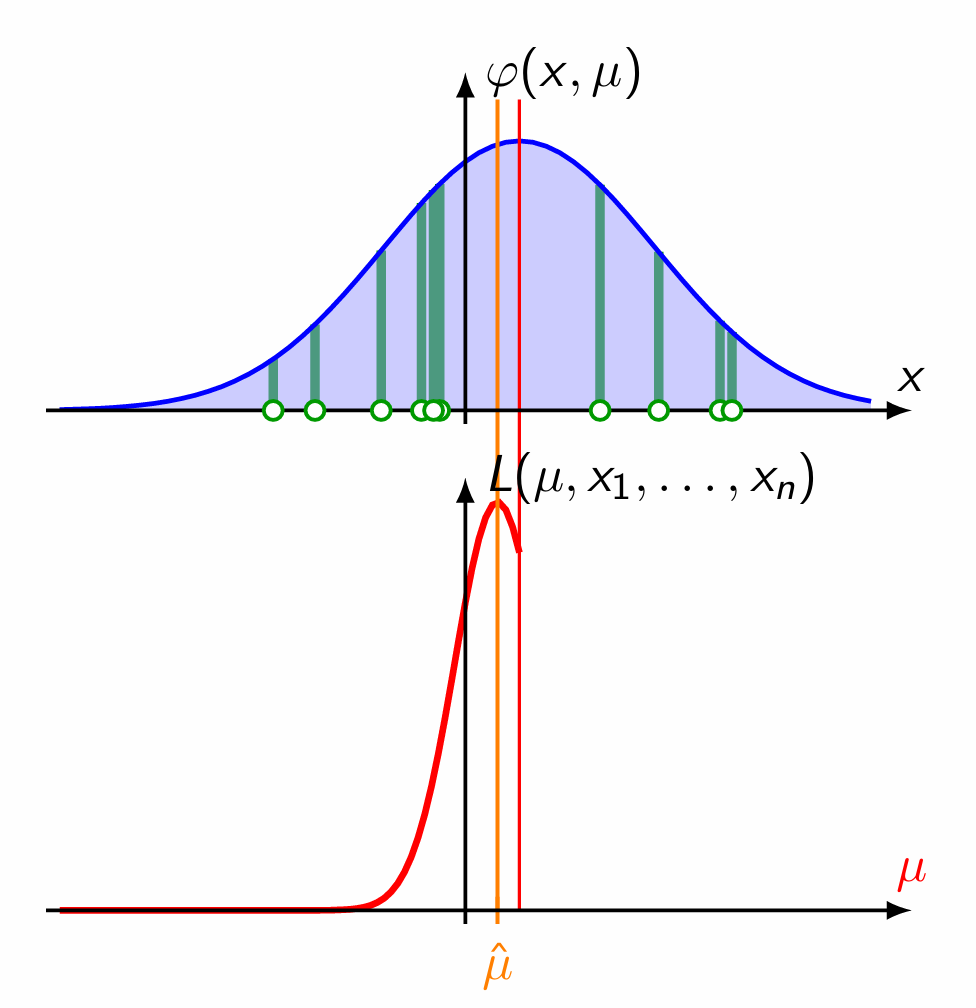
\includegraphics[width=0.5\linewidth]{Images/maximum-likelihood.png}
    \caption{Maximum Likelihood Prinzip}
\end{figure}

\defn{Maximum Likelihood Prinzip}{
    Stichprobe \(x_1,\dots,x_n\) einer Zufallsvariable
    mit Schätzparameter \(\mu\).
    Die Likelihood Funktion bewertet die Kandidaten \(\mu\) mit:
    \begin{equation}
        \begin{split}
            L(\mu,x_1,\dots,x_n) &= \varphi(x_1,\mu)\cdot \dots \cdot\varphi(x_n,\mu) \\
            \hat{\mu} &= argmax(L(\mu, x_1,\dots,x_n)) \text{ für } \mu
        \end{split}
    \end{equation}
    Dies kann man interpretieren als "Wahrscheinlichkeit für die Werte \(x_i\)".
    Die Funktion \(\varphi(x_1,\dots,x_n)\) maximiert \(L\) (Maximum Likelihood Schätzer),
    sodass mit \(\vartheta\) die Messungen \(x_i\) am wahrscheinlichsten sind.
}

\subsection{Korrektur nicht erwartungstreuer Schätzer}
Als erstes muss aus der Schätzer bestimmt werden. Wenn wir erwarten, dass
es sich bei diesen um einen nicht erwartungstreuen Schätzer handelt, muss
der Erwartungswert von \(\varphi(\mu,x_n)\) bestimmt werden. Der Faktor,
welcher mit dem Schätzwert vorhanden ist wird schlussendlich vom beim 
Schätzer eingefügt.
\begin{enumerate}
    \item Maximum Likelihood Prinzip verwenden
    \item Kontrollieren ob dieser erwartungstreu ist (\(E(\hat{b})\))
    \item Kompensationsfaktor verwenden
\end{enumerate}
Grundsätzlich sind Schätzer bereits vorgegeben.

\subsection{Konfidenz-/Vertrauens-Intervall}
Im \([\vartheta_-,\vartheta_+]\) findet man den wahren Wert des
Parameters mit Wahrscheinlichkeit \(1-\alpha\) (Vetrauensniveau):
\begin{enumerate}
    \item Verteilung von \(\hat{\vartheta}\): Wahrscheinlichkeitsdichte
    \(\varphi(\vartheta)\) und Verteilfunktion \(F_\vartheta\)
    \item Finde \(\vartheta\)-Werte so, dass \(1-\alpha=F(\vartheta_-)-F(\vartheta_+)\)
\end{enumerate}

\begin{figure}[H]
    \centering
    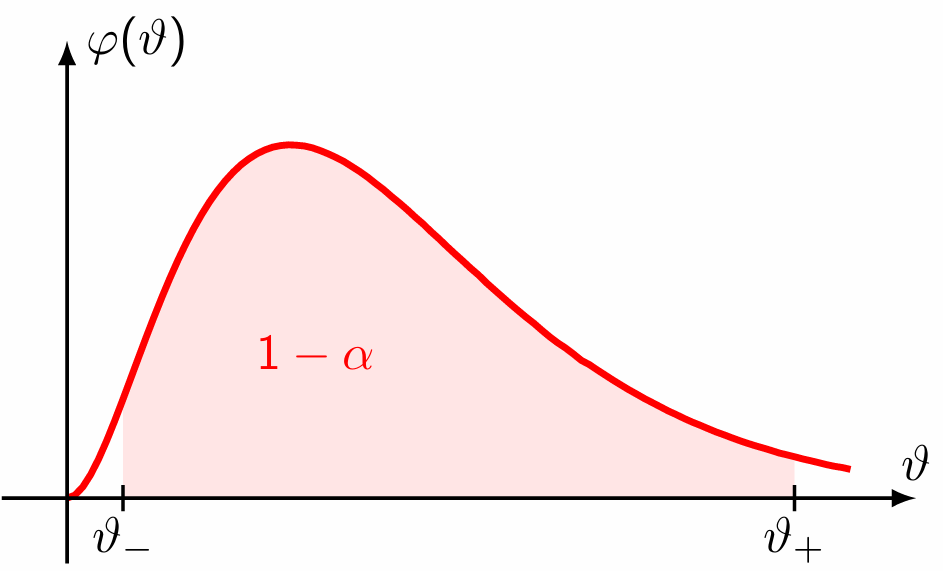
\includegraphics[width=0.5\linewidth]{Images/konfidenzintervall.png}
    \caption{Konfidenzintervall}
\end{figure}



\subsection{Intervallschätzung}
Mit gegebener normalverteilte Stichprobe \(X_i\), lässt sich ein
Intervall finden, welches \(\mu\) mit einer bestimmten Wahrscheinlichkeit enthält.

\begin{equation}
    \hat{\mu} = \frac{1}{n}(X_1+\dots+X_n)
\end{equation} 
Mit \textbf{bekannter Varianz} lässt sich das Intervall einfach schätzen:
\begin{equation}
    [\hat{\mu}-1.96\frac{\sigma}{\sqrt{n}},\hat{\mu}+1.96\frac{\sigma}{\sqrt{n}}]
\end{equation}

Da \(\sigma\) aber vielfach \textbf{unbekannt} ist, lässt sich diese mit der \textbf{T-Verteilung} testen:
\begin{equation}
    t = \frac{\hat{\mu}-\mu}{\hat{\sigma}/\sqrt{n}}
\end{equation} 
Mit der T-Verteilung von \(n-1\) Freiheitsgrade. Das Intevall für 95\% ist dann:
\begin{equation}
    [\hat{\mu}+t_{-}\frac{\sigma}{\sqrt{n}},\hat{\mu}+t_{+}\frac{\sigma}{\sqrt{n}}]
\end{equation}

\exm{Intervall für 95\%}{
    Gesucht ist \(x_{\pm}\) sodass:
    \begin{equation*}
        P(x_{-} \leq X \leq X_{+}) = 0.95
    \end{equation*}
    Durch Standardisierung wird daraus:
    \begin{equation*}
        P(\frac{x_{-}-\mu}{\sigma} \leq \frac{X-\mu}{\sigma} \leq \dots) = 0.95
    \end{equation*}
    Nun kann mittels der Tabelle der Normalverteilung die Werte herausgelesen werden.
}

\section{Hypothesentest}
\subsection{Grundsätzliche Testmethode}
\begin{enumerate}
    \item Nullhypothese \(H_0\) formulieren.
    \begin{itemize}
        \item Nullhypothese \(H_0\)
        \item Alternativhypothese \(H_1\)
    \end{itemize}
    \item Messgrösse bestimmen, mit der \(H_0\) getestet werden kann (Teststatistik)
    \item Verteilung der Messgrösse ermitteln
    \item Parameter der Verteilung schätzen
    \item Kritischen Werte für die Testgrösse bestimmen, der nur mit Wahrscheinlichkeit \(\alpha\) überschritten wird
    \item Ist die Messgrösse im vorliegenden Expermiment "unwahrscheinlich gross"? So verwirft man \(H_0\)
    \begin{itemize}
        \item Kritischer Wert erreicht \(\Rightarrow\) Nullhypothese \(H_0\) verwerfen
    \end{itemize}
\end{enumerate}

\begin{figure}[H]
    \centering
    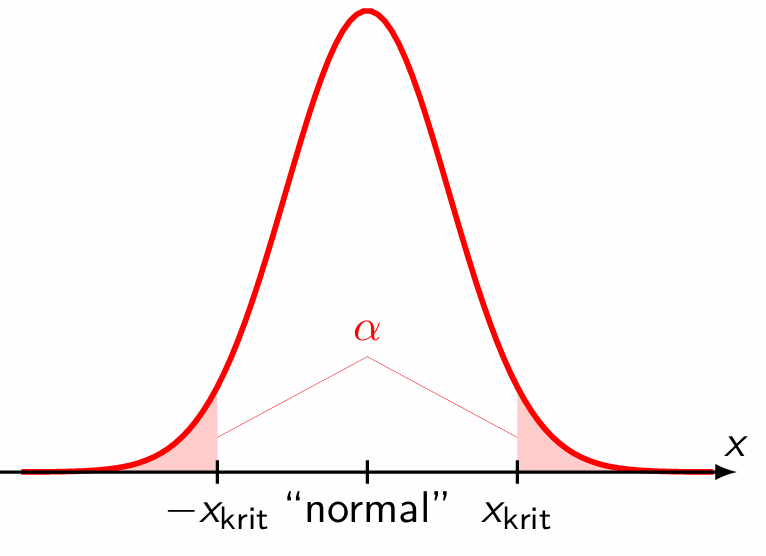
\includegraphics[width=0.5\linewidth]{Images/hypo-test.png}
    \caption{Grundsätzlicher Hypothesentest}
\end{figure}

\subsection{Fehlerarten}
\begin{enumerate}
    \item Nullhypothese verworfen, obwohl dieses wahr ist. Dies passiert wenn zufallsbedingt ein unwahrscheinlicher Wert
    der Teststatistik vorkommt. Es ist ein falsch positives Ergebnis.
    \item Nullhypothese wird nicht verworfen, obwohl dieses falsch ist. Dies ist ein falsch negatives Ergebnis.
\end{enumerate}
Der Fehler 1. tritt mit einer Wahrscheinlichkeit von \(\alpha\) auf.
Die üblichen Werte sind:
\begin{description}
    \item[0.05] signifikant
    \item[0.01-0.001] hoch signifikant 
\end{description}

\subsection{t-Test}
Der Einstichproben-t-Test (englisch one sample t-test) ist ein Signifikanztest aus der mathematischen Statistik.
Er prüft anhand des Mittelwertes einer Stichprobe,
ob der Mittelwert einer Grundgesamtheit gleich einem vorgegebenen Wert ist (bzw. kleiner oder größer).

\defn{t-Test}{
    \begin{equation}
        T = \frac{\bar{X}-\bar{Y}}{\sqrt{(n-1)S_X^2 + (m-1)S_Y^2}} \sqrt{\frac{nm(n+m-2)}{n+m}}
    \end{equation}
    Ist t-Verteilt mit \(m+n-2\) Freiheitsgraden. 
    \begin{equation}
        S_X^2 = \frac{1}{n-1} \sum_{i=1}^{n} (X_i - \bar{X})^2
    \end{equation}
    Für \(S_Y^2\) giltet dieselbe Formel.
}

Wir nehmen an, dass die Streuung der Messwerte der Stichprobe durch die Veränderung des Prozesses
nicht verändert wurde.

Der t-Test auf Gleichheit der Erwartungswerte spielt sich also wie folgt ab. Aus den beiden
Stichproben \(X_1,\dots,X_n\) und \(Y_1,\dots,Y_m\) wird der Ausdruck T gebildet. Übersteigt T den
t-Wert für die \(1-\alpha\)-Quantile der t-Verteilung mit n+m-2 Freiheitsgraden, wird die Hypothese
µ=v verworfen.

\begin{figure}[H]
    \centering
    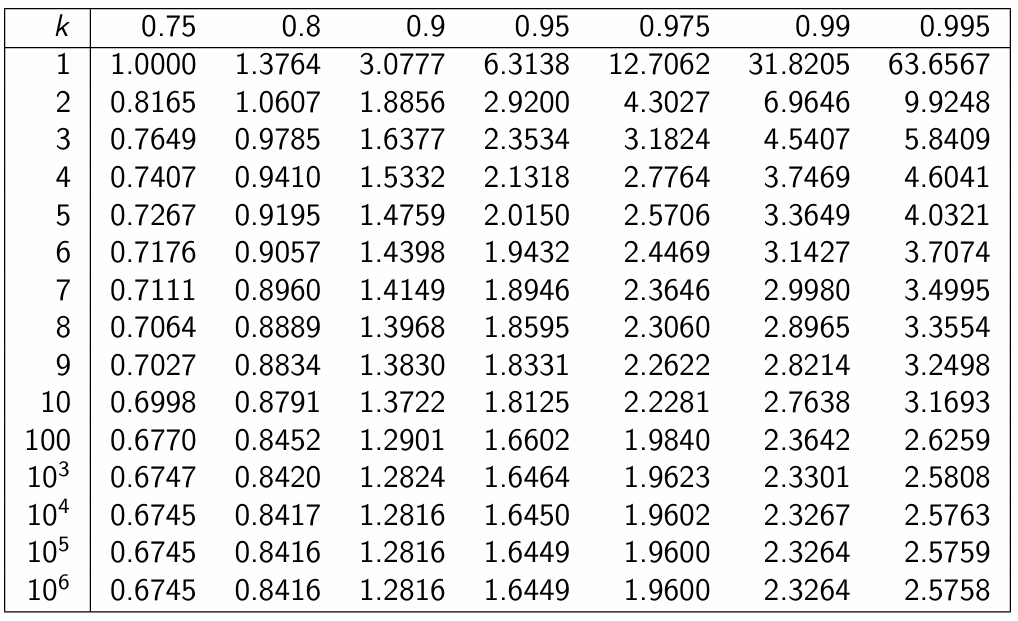
\includegraphics[width=1\linewidth]{Images/t-test-tabelle.png}
    \caption{T-Test Tabelle}
\end{figure}
Dabei beschreibt \(k\) das mit \(m+n-2\) den Freiheitsgrad.

\subsection{p-Value}

\begin{figure}[H]
    \centering
    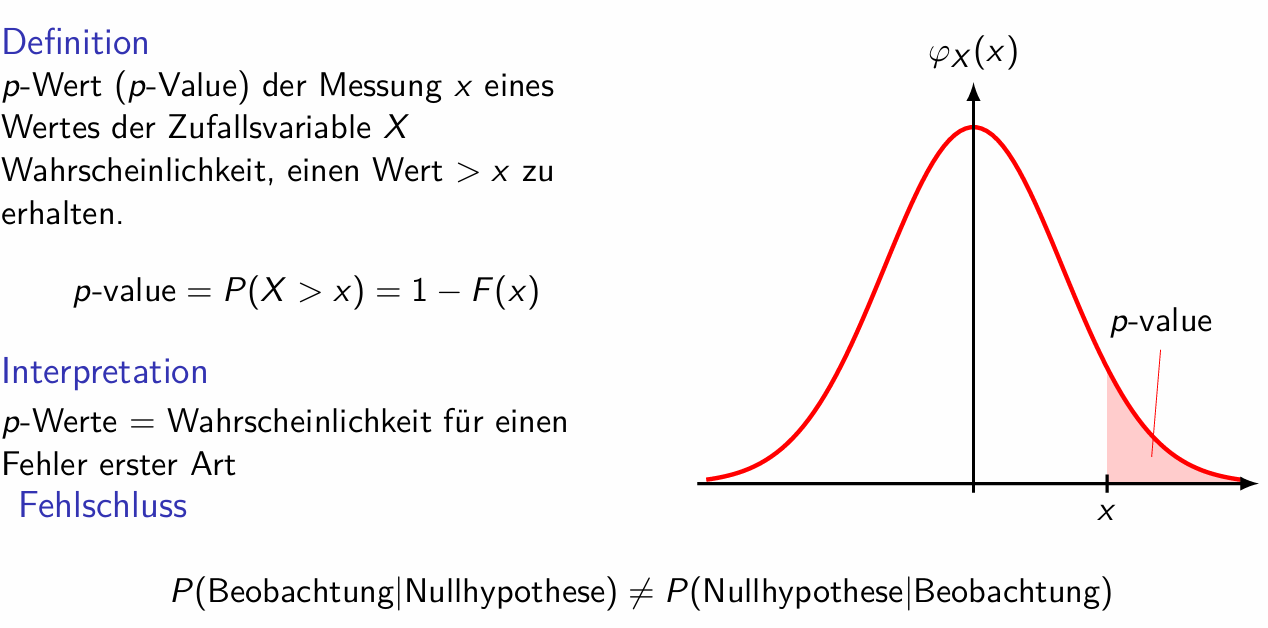
\includegraphics[width=1\linewidth]{Images/p-value.png}
    \caption{p-Value}
\end{figure}

\subsection{Diskrepanz}
Eine verallgemeinerte Testgrösse eines Bernoulli Experiments für
n verschiedene Anzahlen:
\begin{equation}
    D = \sum_{k=1}^{n} \frac{(X_i - np_i)^2}{np_i}
\end{equation}

\begin{figure}[H]
    \centering
    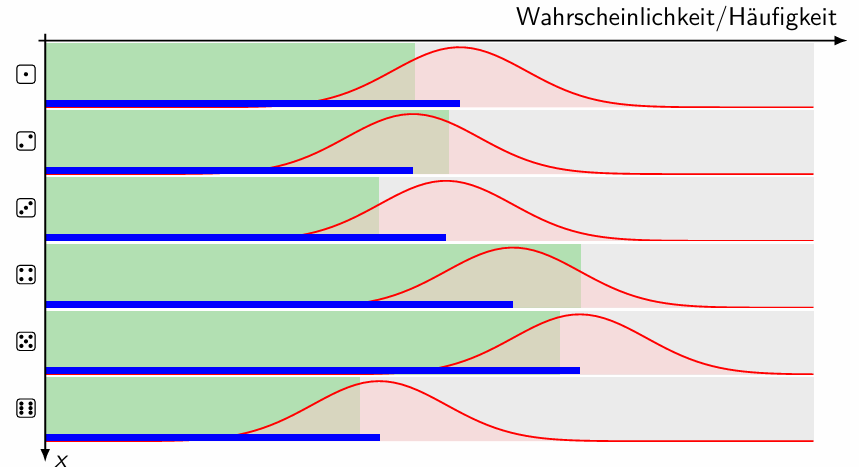
\includegraphics[width=1\linewidth]{Images/hyp-n-anzahl.png}
    \caption{Hypothesentest für Anzahl n}
\end{figure}

\subsection{F-Test TODO unwichtig}

\section{Verteilungstests}
\subsection{\(\chi^2\)-Test}

\begin{figure}[H]
    \centering
    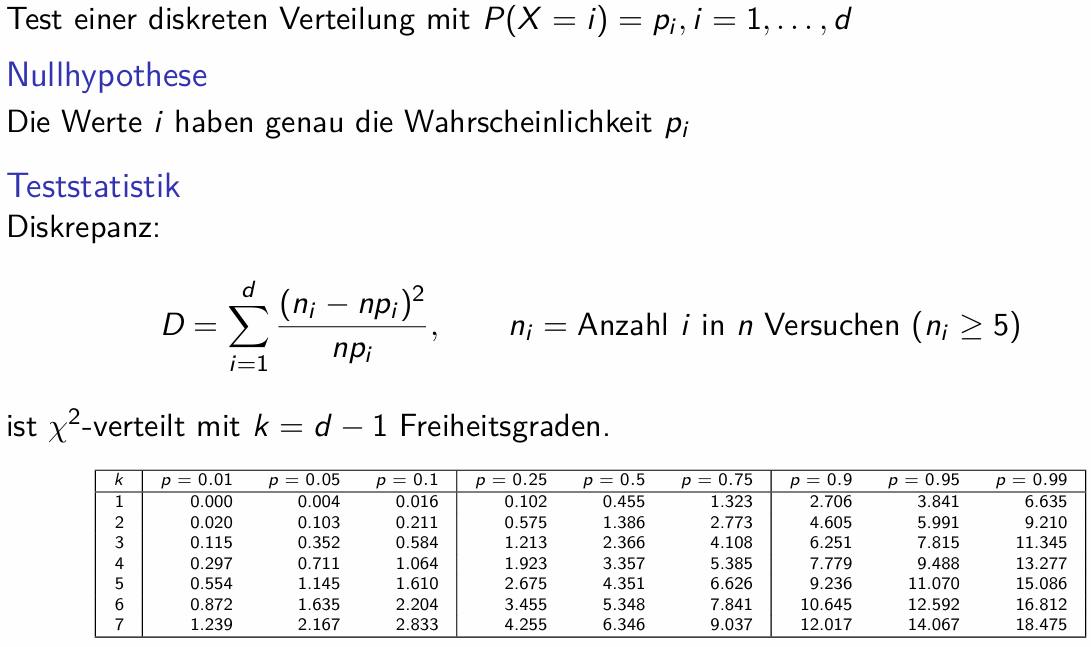
\includegraphics[width=1\linewidth]{Images/x-text.png}
    \caption{Chi Test}
\end{figure}


\begin{figure}[H]
    \centering
    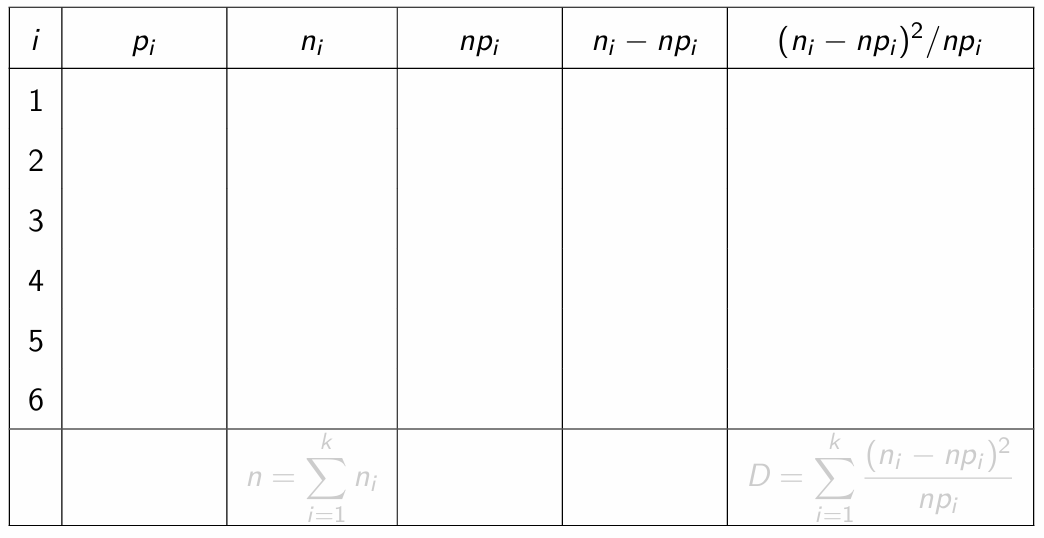
\includegraphics[width=1\linewidth]{Images/diskrepanz-tabelle.png}
    \caption{Chi Diskrepanz Tabelle}
\end{figure}

\begin{figure}[H]
    \centering
    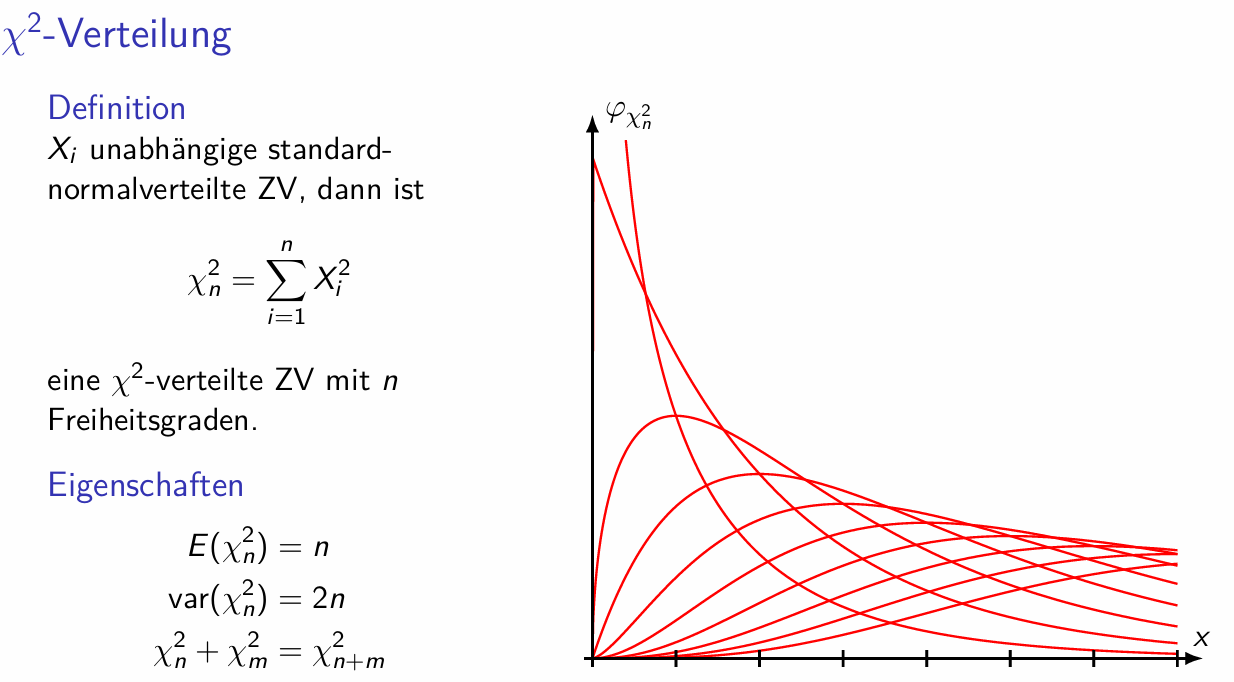
\includegraphics[width=1\linewidth]{Images/x-verteilung.png}
    \caption{Chi Quadrat Verteilung}
\end{figure}

Chi kann auch für zu genaue Ergebnisse testen. Ob gemogelt resp. betrogen wurde.
Der Test funktioniert mit endlich viele Ausgänge.
Der Chi Quadrat test nimmt binomialverteilung für die einzelnen ausgänge.
und diese sind normalapproximiert. das bedeutet, wenn man stetige ausgänge testen
möchte z.b in dem man diese in diskrete klassen zählt, muss man an den rändern aufpassen,
da die normalapproximation für wenige samples schlecht funktioniert.

Faustregel: jede klasse muss mindestens 5 versuchsausgänge haben.

\begin{figure}[H]
    \centering
    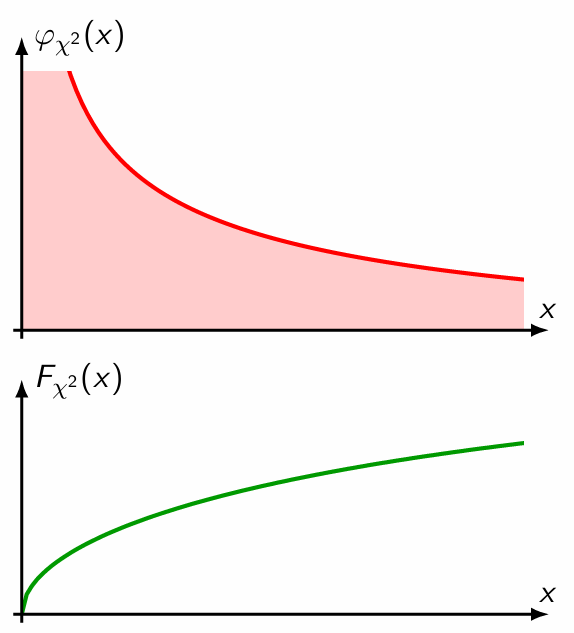
\includegraphics[width=1\linewidth]{Images/chi-verteilung.png}
    \caption{Chi Verteil- und Dichtefunktion}
\end{figure}

\begin{figure}[H]
    \centering
    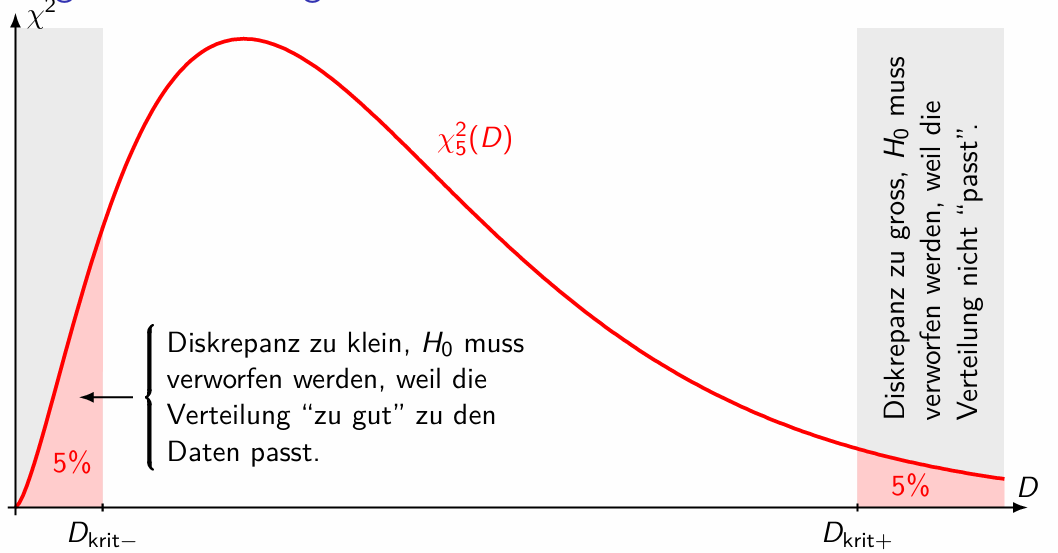
\includegraphics[width=1\linewidth]{Images/chi-gross-klein.png}
    \caption{Chi zu gross oder zu klein?}
\end{figure}

\subsection{Testen einer diskreten Verteilung}

\begin{figure}[H]
    \centering
    \includegraphics[width=1\linewidth]{Images/test-diskrete-verteilung.png}
    \caption{Testen einer diskreten Verteilung}
\end{figure}
K = Anzahl der Ausgänge minus eins. (auch Freiheitsgrade genannt)

\begin{figure}[H]
    \centering
    \includegraphics[width=1\linewidth]{Images/beispiel-hyp-faire-münze.png}
    \caption{Beispiel: Testen einer fairen Münze}
\end{figure}

\begin{figure}[H]
    \centering
    \includegraphics[width=1\linewidth]{Images/beispiel-hyp-mittelwert.png}
    \caption{Beispiel: Testen von zwei Mittelwerte}
\end{figure}

\section{Filter}
\defn{Filtern}{
    Aus fehlerbehafteten Beobachtungen eines dynamischen Systems die
    aktuellen Parameter des Systens optimal, d.h. mit kleinstmöglichem
    Fehler schätzen.
    \begin{equation}
        \hat{\mu} = \frac{X_1+\dots+X_n}{n}
    \end{equation}

    Dabei ist aber meistens die Einzelmessung
    \(X_i\) nicht die einzige Informationsquelle
    üver den Systemzustand \(\hat{\mu}\)
}

\begin{figure}[H]
    \centering
    \includegraphics[width=0.25\linewidth]{Images/schaetzen.png}
    \caption{Schätzen des Systemzustandes mithilfe des Systemmodells}
\end{figure}
Um erfolgreich zu schätzen, möchten wir also
zusätzliche Informationen beiziehen um ein
statistisches Problem zu lösen.

\subsection{Optimaler Schätzer für zwei Messgrössen}
Gegeben ist ein Problem mit zwei Zufallsvariabeln
\(X_1,X_2\), welche dieselbe grösse Messen.
Sie sind unabhängig und besitzen unterschiedliche
Varianz resp. Messfehler \(var(X_i)=\sigma_i^2\).
Um die gesamte Information zu verwenden benutzen
wir gewichtete Variabeln mit \(X\):
\begin{equation}
    \begin{split}
        X &= tX_1+(1-t)X_2 \\
        var(X) &= t^2var(X_1) + (1-t)^2var(X_2)
    \end{split}
\end{equation}
Nun wird die Linearkombination so gewählt,
dass \(var(X)\) minimal wird.
Dies geschieht durch das Null-Setzen der Ableitung nach \(t\) mit: \(\frac{d}{dt}var(X)=0\).
\defn{Optimale Faktoren für zwei Messgrössen mit unterschiedlichem Fehler}{
    \begin{equation}
        \begin{split}
            t &= \frac{\sigma_2^2}{\sigma_1^2+\sigma_2^2} \\
            \hat{\mu}(X_1,X_2) &= \frac{\sigma_2^2}{\sigma_1^2+\sigma_2^2}X_1+\frac{\sigma_1^2}{\sigma_1^2+\sigma_2^2}X_2\\
            \text{Fehler: } var(\hat{\mu}) &= \frac{\sigma_1^2 \sigma_2^2}{\sigma_1^2+\sigma_2^2}
        \end{split}
    \end{equation}
}
Für den zweiten Sensor nähme man: \(t_2 = 1-t\).
Wenn also z.B. \(\sigma_2^2\) sehr gross ist, nähert
sich der Ausdruck 1 an. Sprich der erste Sensor
wir stärker gewichtet, wenn der Messfehler des Zweiten grösser ist.


\begin{figure}[H]
    \centering
    \includegraphics[width=1\linewidth]{Images/verbesserung-genauigkeit-filter.png}
    \caption{Genauigkeitsverbesserung durch den Messwert \(X_2\)}
\end{figure}
\newpage

\subsection{Rauchen in einem Kanal}
Gegeben ist ein Eingangssignal \(X\) welches durch ein Rauchen gestört wird.
Man möchte nun mit zwei Verstärkungsfaktoren \(a,b\) versuchen das Rauschen zu minimieren.
In dem das Signal mit den gewöhnlichen Tönen verstärkt wird und schlussendlich wieder gedämpft.
\(A,b\) kontrolliert die Verstärkung oder Dämpung des Signals bei den Einheiten.
\\\\
Das Ziel ist nun also \(b\) so zu wählen, damit die Varianz von \(\Delta=Y-X\) minimal wird.

\begin{figure}[H]
    \centering
    \includegraphics[width=0.5\linewidth]{Images/wiener-filter.png}
    \caption{Wiener-Filter für Rauschminimierung}
\end{figure}

Durch das Minimieren der Varianz können die optimalen Faktoren bestimmt werden:
\begin{equation}
    \begin{split}
        var(\Delta) &= var(b(aX+N)-X)\\
        &\Rightarrow \frac{d}{db}var(\Delta)
    \end{split}
\end{equation}

\defn{Wiener-Filter}{
    \begin{equation}
        \begin{split}
            b &= \frac{a\sigma^2}{a^2\sigma^2+\sigma_2^2} \\
            \text{Fehler: } var(\Delta) &= \frac{\sigma_N^2}{a^2+\sigma_N^2/\sigma^2}
        \end{split}
    \end{equation}
}
\(\frac{\sigma_N^2}{\sigma^2}\) heisst auch "Signal-Rauschabstand", wobei Zähler
die Grössenordnung des Rauschens und der Nenner die des Signals ist.
Diese Art von Filterung ist einer der einfachsten, jedoch nicht optimal, da
die Qualität von den Frequenzen abhängen.

\subsection{Frequenzabhängige Filterung}
Das Verhältnis zwischen Rauschen und Signal ist unterschiedlich je nach Frequenz.
Es ist nicht ausreichend für jede Frequenz das gleiche B zu wählen.

\subsection{Systembeschreibung}
\subsection{Fehler}
\subsection{Kovarianz Matrix}

\section{Aufgaben Lösen}
\begin{enumerate}
    \item Welche Zufalls grössen liegen vor?
    \item Welche Art von Zufalls prozess erzeugt die Zufallsgrösse?
    \item Welche Parameterwerte müssen verwendet werden? (Schätzen)
    \item Wahrscheinlichkeiten berechnen
\end{enumerate}

\end{document}

